\documentclass[utf8]{ctexart} %中文文档类
\usepackage[left=2.50cm, right=2.50cm, top=2.50cm, bottom=2.50cm]{geometry} % 页边距
\usepackage{indentfirst} % 首行缩进
\usepackage{fancyhdr} % 设置页眉、页脚
\renewcommand\headrulewidth{0pt}% 页眉与正文之间的水平线粗细
\usepackage{ctexcap} % 标题是中文的
\usepackage{helvet} % 用来指定beamer使用的字体
\usepackage{hyperref} % bookmarks 
\usepackage{multicol} % 分栏

\usepackage{amsmath, amsfonts, amssymb} % 数学公式、符号
\usepackage[english]{babel} % 数学公式标准
\usepackage{bm} % 加粗方程字体 
\usepackage{float}

\usepackage{graphicx} % 图片 
\usepackage{svg}
% \svgsetup{
%     inkscapepath=i/svg-inkscape/
% }
% \svgpath{{svg/}}

\svgsetup{inkscapelatex=false} % keep original font and size
\usepackage{url} % 超链接 

\usepackage{multirow} % 表格
\usepackage{booktabs} % 三线表
\usepackage{longtable} % 长表格

%\usepackage{algorithm} % 算法或伪代码
%\usepackage{algorithmic} % 算法或伪代码
\usepackage[linesnumbered,lined,boxed,commentsnumbered]{algorithm2e}

\usepackage{enumitem} % 枚举环境宏包

%\renewcommand{\algorithmicrequire}{ \textbf{Input:}} 
%\renewcommand{\algorithmicensure}{ \textbf{Initialize:}} 
%\renewcommand{\algorithmicreturn}{ \textbf{Output:}} %算法格式

\newtheorem{theorem}{\indent 定理}[section]
\newtheorem{lemma}[theorem]{\indent 引理}
\newtheorem{proposition}[theorem]{\indent 命题}
\newtheorem{corollary}[theorem]{\indent 推论}
\newtheorem{definition}{\indent 定义}[section]
\newtheorem{example}{\indent 例}[section]
\newtheorem{remark}{\indent 注}[section]
\newenvironment{solution}{\begin{proof}[\indent\bf 解]}{\end{proof}}
\renewcommand{\proofname}{\indent\bf 证明}

\pagestyle{fancy} \lhead{} \chead{} \lfoot{} \cfoot{} \rfoot{}
\pagestyle{plain}
\hypersetup{colorlinks, bookmarks, unicode} % unicode 
 
\title{\textbf{Euler B\`{e}zier 曲线与Euler B-Spline曲线}}
\author{\bf 王庶霖}
\date{}

\hypersetup{
colorlinks=true,
linkcolor=black
} % 使目录为黑色字
\counterwithin{figure}{section}
\numberwithin{figure}{section}

\begin{document}  
		\maketitle
		\renewcommand{\contentsname}{目录} 
		\tableofcontents
		\newpage 
		\renewcommand{\abstractname}{\Large 摘要}

		\begin{abstract}
		\addcontentsline{toc}{section}{摘要}
		\normalsize
		这里是摘要内容。这里是摘要内容。这里是摘要内容。这里是摘要内容。这里是摘要内容。这里是摘要内容。这里是摘要内容。这里是摘要内容。

		\noindent{\bf 关键词: }关键词1 关键词2 关键词3 ... 
		\end{abstract}
		\newpage  
		\section{平面Euler B\'{e}zier曲线与Euler B-Spline曲线}
		
		\begin{definition}[Euler 多边形]\label{EP2D}
			如果平面多边形$\boldsymbol{P}_0\dots\boldsymbol{P}_n$满足
			\begin{equation}
				\begin{aligned}
					&(1).\quad \Arrowvert\boldsymbol{P}_i\boldsymbol{P}_{i+1}\Arrowvert(i=0,1,\dots,n-1)\text{是定值};\\
					&(2).\quad\theta_i(i=1,2,\dots,n-1)\text{是等差数列},
				\end{aligned}
			\end{equation}
			则称该多边形为Euler多边形.
		\end{definition}
	\begin{definition}[Euler B\'{e}zier曲线]\label{EB_Def}
		如果平面B\'{e}zier曲线$\boldsymbol{P}(t)=\sum_{i=0}^n\boldsymbol{P}_iB_{i,n}(t), t\in[0,1]$的控制多边形是Euler多边形, 则称曲线$\boldsymbol{P}(t)$是Euler B\'{e}zier曲线. 
	\end{definition}
		\begin{definition}[Euler B-Spline 曲线]\label{Esp_Def}
			记平面上的$k$阶均匀节点B-Spline曲线$\boldsymbol{P}(t)=\sum_{i=0}^n\boldsymbol{P}_iN_{i,k}(t), t\in[t_{k-1},t_{n+1}]$,节点向量$t_i = i\quad(i=0,1,\dots,n+k)$. 如果其控制多边形$\boldsymbol{P}_i$是Euler多边形, 则称曲线$\boldsymbol{P}(t)$是Euler B-Spline曲线.
		\end{definition}
		
		\begin{figure}[htbp]
			\centering
			\begin{minipage}{0.49\linewidth}
				\centering
				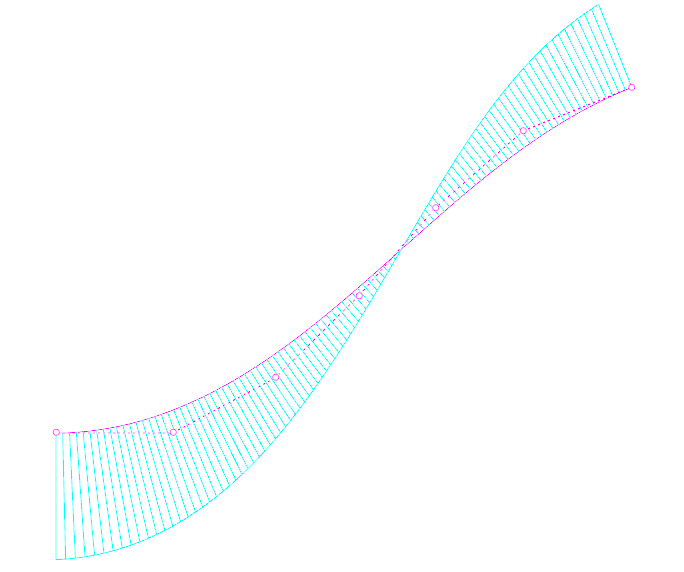
\includegraphics[width=0.9\linewidth]{figures/EulerBezierDef1.png}
			\end{minipage}
			%\qquad
			\begin{minipage}{0.49\linewidth}
				\centering
				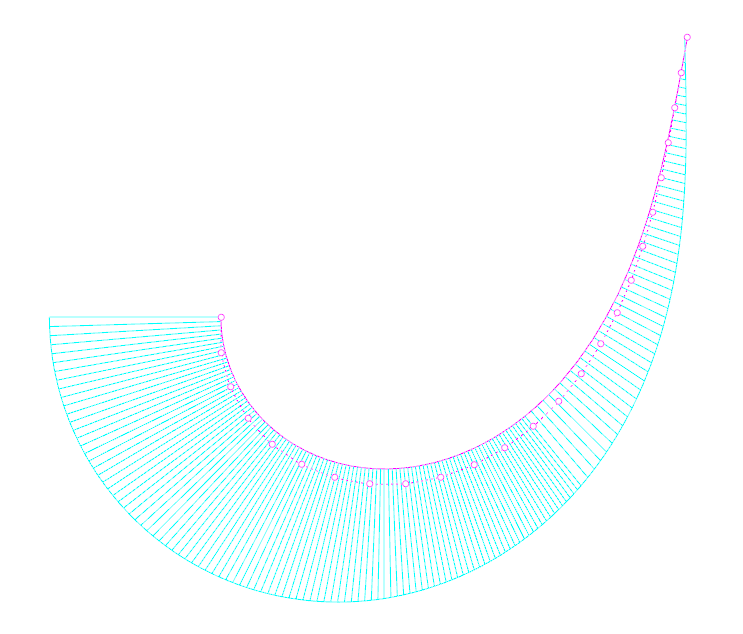
\includegraphics[width=0.9\linewidth]{figures/EulerBezierDef2.png}
			\end{minipage}
			\caption{Euler Bezier曲线}
		\end{figure}
		
		
		\section{利用Euler B\'{e}zier曲线和Euler B-Spline曲线构造G2连续圆角曲线}
		\subsection{平面Euler B\'{e}zier曲线}
		对于一个给定的多边形, 对转角做圆角处理是非常常见的需求, 传统的方法是使用圆弧, 通过确定圆弧的半径来控制圆角的程度. 由于圆弧是固定曲率的, 这种传统的方法只能构造$G^1$连续的圆角, 使用Euler B\'{e}zier曲线则可以构造出$G^2$连续的圆角曲线, 并且可以保证有且仅有一个曲率极值点.\par
		考虑多边形的一个转角$\boldsymbol{ABC}$, 向量$\boldsymbol{AB}$到向量$\boldsymbol{BC}$的旋转角为$\alpha, |\alpha|\in(0,\pi)$, 我们对转角$\boldsymbol{B}$构造圆角曲线. 由于Euler B\'{e}zier螺线是曲率单调的, 而多边形的圆角曲线要达到$G^2$连续需要保证两端的曲率为0, 所以我们使用对称的两条Euler B\'{e}zier螺线拼接得到圆角曲线. 设圆角曲线的起点$\boldsymbol{P}_S$在边$\boldsymbol{AB}$上, 由于要构造对称的两条曲线, 我们把一边曲线的终点$\boldsymbol{P}_E$取在多边形的内角平分线上. 为保证$G^1$连续, 起点$\boldsymbol{P}_S$处的切方向为向量$\boldsymbol{AB}$的方向, 记为$\boldsymbol{T}_S = \boldsymbol{AB}/\Arrowvert\boldsymbol{AB}\Arrowvert$. 终点$\boldsymbol{P}_E$处的切向$\boldsymbol{T}_E$应当与多边形的内角平分线垂直. 假设B\'ezier曲线$\boldsymbol{P}(t)=\sum_{i=0}^n\boldsymbol{P}_iB_{i,n}(t),t\in[0,1]$插值了这两个边界条件, $\boldsymbol{P}_i\boldsymbol{P}_{i+1}$到$\boldsymbol{P}_{i+1}\boldsymbol{P}_{i+2}$的角为$\theta_{i+1}(i=0,1,\dots,n-2)$. 那么可以得到
		\begin{equation}
			\prod_{i=1}^{n-1}\text{R}(\theta_i)\boldsymbol{T}_S =  \boldsymbol{T}_E
		\end{equation}
		其中$\text{R}(\theta)$表示旋转角为$\theta$的旋转矩阵. 根据定义($\ref{EB_Def}$), $\theta_i$应当为等差数列. 考虑B\'ezier曲线的起点曲率$$\kappa(0)=\frac{n-1}{n}\frac{\sin(\theta_1)}{l}$$
		保证$G^2$连续要令$\kappa(0)=0$, 则有$\theta_1=0$, 故设$\theta_i=(i-1)\Delta\theta(i=1,\dots,n-1)$, 为了保证对称性, $\boldsymbol{T}_E$应当与多边形内角平分线垂直, 则$\boldsymbol{T}_S$到$\boldsymbol{T}_E$的夹角为$\alpha/2$, 所以有
		\begin{equation}
			\sum_{i=1}^{n-1}\theta_i = \frac{(n-2)(n-1)}2\Delta\theta = \frac{\alpha}2
		\end{equation}
		计算得$\Delta\theta=\frac{\alpha}{(n-2)(n-1)}$, 从而计算每个$\theta_i$. Euler多边形顶点的序列可以递推给出:
		\begin{equation}\label{recur}
			\begin{aligned}
				\boldsymbol{P}_0\boldsymbol{P}_1 &=l\boldsymbol{T}_S\\
				\boldsymbol{P}_1\boldsymbol{P}_2 &=\text{R}(\theta_1)\boldsymbol{P}_0\boldsymbol{P}_1\\
				\dots\\
				\boldsymbol{P}_i\boldsymbol{P}_{i+1} &=\text{R}(\theta_i)\boldsymbol{P}_{i-1}\boldsymbol{P}_i
			\end{aligned}
		\end{equation}
		根据起点终点条件有$\boldsymbol{P}_0=\boldsymbol{P}_S, \boldsymbol{P}_n = \boldsymbol{P}_E$, 结合递推式($\ref{recur}$)得到:
		\begin{equation}
			\boldsymbol{P}_S\boldsymbol{P}_E = \sum_{i=0}^{n-1}\boldsymbol{P}_i\boldsymbol{P}_{i+1} = l[\sum_{i=0}^{n-1}\text{R}(\phi_i)]\boldsymbol{T}_S
		\end{equation}
		其中$\phi_i=\sum_{j=1}^i\theta_j (i = 1,\dots,n-1), \phi_0 = 0$. 对于一个给定正整数$n$, 我们可以计算出向量$\boldsymbol{D} = \sum_{i=0}^{n-1}\text{R}(\phi_i)\boldsymbol{T}_S$, 这是一个常向量, 从起点到终点的连线必须与它平行. 将向量$\boldsymbol{D}$与向量$\boldsymbol{T}_S$的夹角记为$\beta$(注意$\beta$也是有符号角, 应当与$\alpha$符号相同), 则有
		\begin{equation}\label{sinthoery}
			\frac{\Arrowvert\boldsymbol{OP}_S\Arrowvert}{\cos(\frac{\alpha}2-\beta)}=\frac{\Arrowvert\boldsymbol{OP}_E\Arrowvert}{\sin(\beta)}=\frac{\Arrowvert\boldsymbol{P}_S\boldsymbol{P}_E\Arrowvert}{\cos(\frac{\alpha}2)}
		\end{equation}
		根据方程$(\ref{sinthoery})$, 我们可以在给定圆角起点$\boldsymbol{P}_S$或者给定角平分线上的经过点$\boldsymbol{P}_E$时求得唯一的Euler多边形. 对于n+1个顶点的Euler多边形, 判断以它们为控制顶点的B\'{e}zier曲线是否为Euler B\'{e}zier曲线, 如果没有满足Euler B\'{e}zier曲线的条件, 则使n自加一再次重复上述过程, 直到满足Euler B\'{e}zier曲线的条件或者控制顶点数达到了预先设定的最大值停止迭代. 如果迭代结束曲线满足了螺线条件, 就得到了一半的圆角曲线. 再将该曲线沿着转角的平分线作对称变换即可得到另一半圆角曲线, 该算法的伪代码实现见Algorithm \ref{smoothcurve1}.\par 
		图(\ref{EB_figure})是对正六边形(黑色直线段)应用Algorithm \ref{smoothcurve1}的结果, 六个圆角曲线(品红色)均为对称的两条四次B\`ezier曲线拼接而成, 其圆角起点与终点都是六边形边的三等分点. 图中的浅蓝色曲率梳表明了该圆角的$G^2$连续性, 并且每一个圆角曲线自身对称, 有且仅有一个曲率极值点, 位于对称轴上.
		\IncMargin{1em}
		 \begin{algorithm}
		 	\SetKwData{Left}{left}\SetKwData{This}{this}\SetKwData{Up}{up}
		 	\SetKwFunction{Union}{Union}\SetKwFunction{FindCompress}{FindCompress}
		 	\SetKwInOut{Input}{input}\SetKwInOut{Output}{output}
		 	\caption{Euler B\'{e}zier圆角}\label{smoothcurve1}
		 	\KwData{ 构成Corner的三个顶点$\boldsymbol{A},\boldsymbol{B},\boldsymbol{C}$, $\boldsymbol{BP}_S$的长度$L_S$或$\boldsymbol{BP}_E$的长度$L_E$}
		 	\KwResult{
		 	B\'ezier曲线$\boldsymbol{P}(t)$的控制顶点序列$\boldsymbol{P}_0,\boldsymbol{P}_1,\dots,\boldsymbol{P}_n$和对称的顶点序列}
		 	\BlankLine 
		 	 $n=4$\;
		 	 \bf{初始化B\'{e}zier曲线}$\boldsymbol{P}(t)$\;
		 	$\boldsymbol{T}_S = \text{Normalize}(\boldsymbol{B}-\boldsymbol{P}_S)$\;
		 	$\boldsymbol{D}=\boldsymbol{T}_S$\;
		 	$\boldsymbol{temp}=\boldsymbol{T}_S$\;
		 	
		 	\While{\text{EulerB\'{e}zierSpiralCheck}($\boldsymbol{P}(t)$)==\text{FALSE} and $n < 20$}{
	计算$\boldsymbol{A}\boldsymbol{B}$与$\boldsymbol{B}\boldsymbol{C}$的夹角$\alpha$\;
		 	$\Delta\theta = \frac{\alpha}{ (n - 2)  (n - 1)}$\;
		 	\For{$i=0,1,\dots,n-2$}{
		 	$\boldsymbol{temp}.\text{Rotate}(i*\Delta\theta)$\;
		 	$\boldsymbol{D}+=\boldsymbol{temp}$\;
		 }
		 	计算$\boldsymbol{A}\boldsymbol{B}$与$\boldsymbol{D}$的夹角$\beta$\;
		 	$\text{length} = \cos(\alpha / 2) / \cos(\alpha / 2 - \beta) * \Arrowvert\boldsymbol{B} - \boldsymbol{P}_S\Arrowvert / \Arrowvert \boldsymbol{D}\Arrowvert$\;
		 	$\boldsymbol{temp}=\boldsymbol{T}_S*\text{length}$\;
		 	$\boldsymbol{P}_0=\boldsymbol{P}_S$\;
		 	\For{$i=1,\dots,n-1$}{
		 	$\boldsymbol{P}_i=\boldsymbol{P}_{i-1}+\boldsymbol{temp}$\;
		 	$\boldsymbol{temp}.\text{Rotate}((i-1)*\Delta\theta)$\;
		 }
		 	$n++$\;
		 }
		 \end{algorithm}
		 \begin{figure}[htbp]
		 	\centering
		 	\begin{minipage}{0.49\linewidth}
		 		\centering
		 		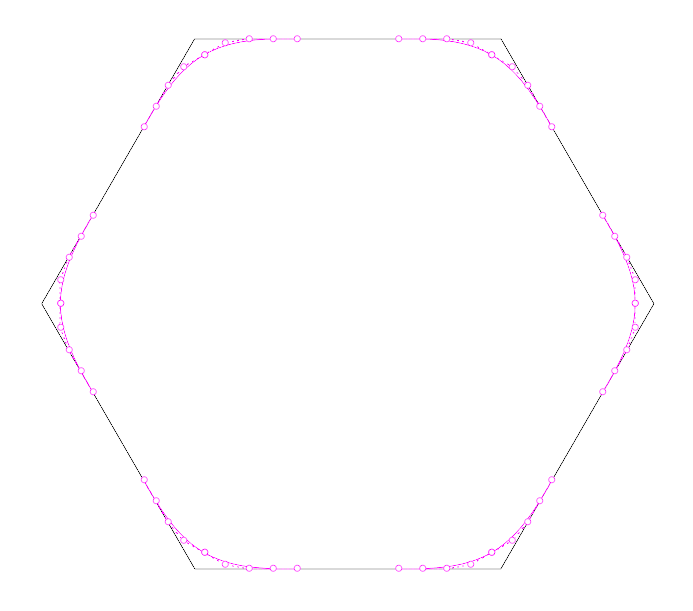
\includegraphics[width=0.9\linewidth]{figures/SmoothCorner1.png}
		 	\end{minipage}
		 	%\qquad
		 	\begin{minipage}{0.49\linewidth}
		 		\centering
		 		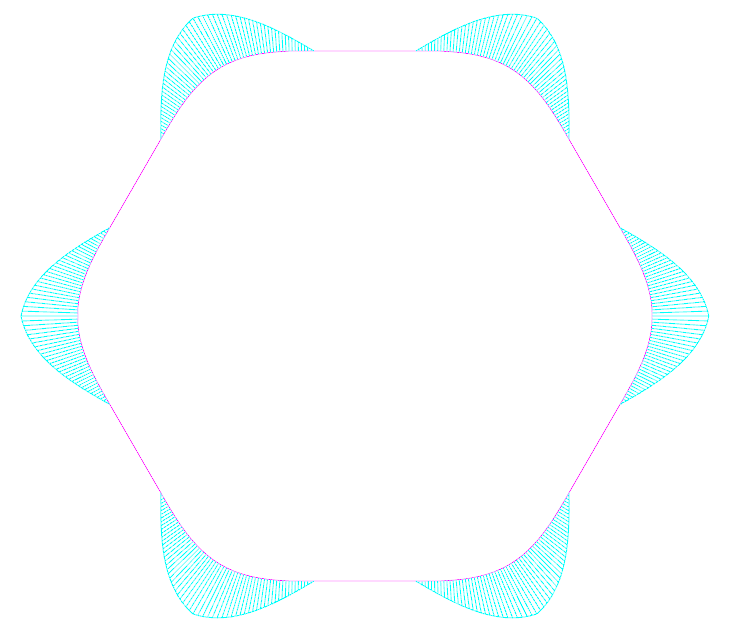
\includegraphics[width=0.9\linewidth]{figures/SmoothCorner2.png}
		 	\end{minipage}
	 	
		 	\caption{算法($\ref{smoothcurve1}$)得到的$G^2$连续Euler B\`{e}zier螺线圆角}
		 	\label{EB_figure}
		 \end{figure}
	 \begin{figure}[htbp]
	 	\centering
	 	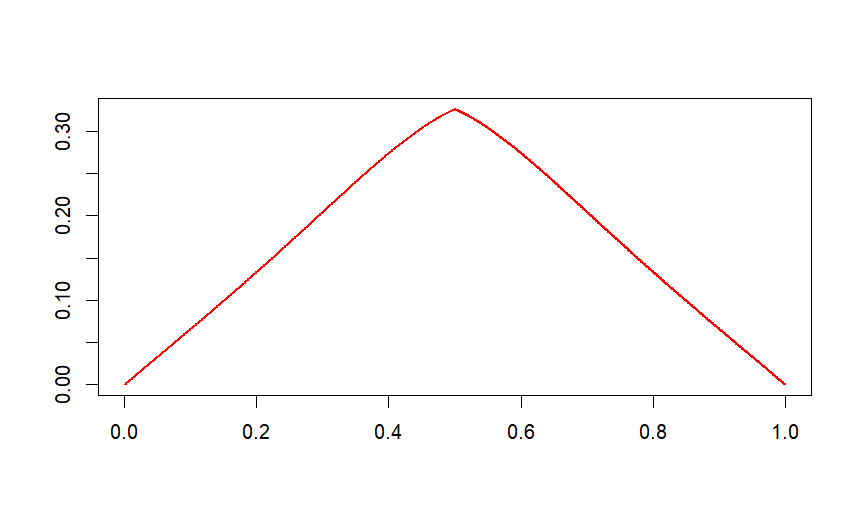
\includegraphics[width=0.7\linewidth]{figures/SixEdges_EulerBezier.png}
	 	\caption{图(\ref{EB_figure})中一个圆角曲线的曲率. }
	 \end{figure}
	 \subsection{平面Euler B-Spline曲线}
	 虽然B\'ezier曲线已经能得到满足条件的圆角曲线, 但是通常控制顶点较多导致次数较高, 而使用B-Spline曲线可以保持次数为三次, 方便进行曲线的拼接处理. 利用二维Euler B-Spline曲线构造圆角大体与B\'{e}zier曲线的构造一致, 只是生成Euler多边形时考虑不同的边界条件.  设四阶(三次)均匀B-Spline 曲线为$\boldsymbol{P}(t)=\sum_{i=0}^n\boldsymbol{P}_iN_{i,4}(t)$, 节点向量为$t_j = j,j=0,1,\dots,n+4$ \par 
	 在Euler B\'{e}zier圆角的构造中, 我们将起点$\boldsymbol{P}_0$设置在圆角起点$\boldsymbol{P}_S$上, 我们令向量$\boldsymbol{P}_0\boldsymbol{P}_1$与$\boldsymbol{T}_S$同向, 令$\boldsymbol{P}_0$$\boldsymbol{P}_1$$\boldsymbol{P}_2$三点共线, 这些都是基于B\'{e}zier曲线的端点各阶导数与控制顶点的关系得到的. 而对于所求的均匀节点B-Spline曲线$\boldsymbol{P}(t)$, $t\in[3,n+1]$, 我们有
	 \begin{equation}
	 \begin{aligned}
	 &\boldsymbol{P}(3)=\frac{\boldsymbol{P}_0+4\boldsymbol{P}_1+\boldsymbol{P}_2}6\\
	 &\boldsymbol{P}'(3)=\frac{\boldsymbol{P}_2-\boldsymbol{P}_0}2\\
	 &\boldsymbol{P}''(3)=\boldsymbol{P}_0-2\boldsymbol{P}_1+\boldsymbol{P}_2
	 \end{aligned}
	 \end{equation}
	 为满足$G^2$连续条件, 必须有
	 \begin{equation}\label{EBS_condition}
	 \begin{aligned}
	 &\frac{\boldsymbol{P}_0+4\boldsymbol{P}_1+\boldsymbol{P}_2}6=\boldsymbol{P}_S\\
	 &\boldsymbol{P}_2-\boldsymbol{P}_0=\lambda\boldsymbol{T}_S\text{, for some }\lambda>0\\
	 &\boldsymbol{P}_0\boldsymbol{P}_2\times(\boldsymbol{P}_1\boldsymbol{P}_2-\boldsymbol{P}_0\boldsymbol{P}_1)=\boldsymbol{0}
	 \end{aligned}
	 \end{equation}
	 第三个条件等价于$\boldsymbol{P}_0\boldsymbol{P}_2\times\boldsymbol{P}_0\boldsymbol{P}_1=\boldsymbol{0}$, 所以等式成立当且仅当$\boldsymbol{P}_0,\boldsymbol{P}_1$与$\boldsymbol{P}_2$三点共线. 注意到Euler多边形各边等长,  故方程(\ref{EBS_condition})的解为
	 \begin{equation}\label{Solution}
	 \left\{
	 \begin{aligned}
	 &\boldsymbol{P}_0 = \boldsymbol{P}_S-l\boldsymbol{T}_S\\
	 &\boldsymbol{P}_1 = \boldsymbol{P}_S\\
	 &\boldsymbol{P}_2 = \boldsymbol{P}_S+l\boldsymbol{T}_S
	 \end{aligned}
	 \right.
	 \end{equation}
	 其中$l>0$为多边形的边长.\par 
	 另外$\Delta\theta$与常向量$\boldsymbol{D}$的定义也会发生变化, 由于终点的导数为
	 \begin{equation}
	 \boldsymbol{P}'(n+1) = \frac{\boldsymbol{P}_n-\boldsymbol{P}_{n-2}}2
	 \end{equation}
	 所以$\theta_i$与$\alpha$的关系变为
	 \begin{equation}
	 \sum_{i=2}^{n-2}\theta_i+\frac12\theta_{n-1}=\frac{\alpha}2
	 \end{equation}
	 结合$\theta_i=(i-1)\Delta\theta$, 得到
	 \begin{equation}
	 \Delta\theta = \frac{\alpha}{(n-2)^2}
	 \end{equation}
	 记$\phi_i=\sum_{j=1}^i\theta_j (i = 1,\dots,n-1), \phi_0 = 0$. 可以表示控制多边形每一个顶点的坐标
	 \begin{equation}\label{recursive_bspline}
	 \boldsymbol{P}_k = \boldsymbol{P}_0+l\sum_{i=0}^{k-1}\text{R}(\phi_i)\boldsymbol{T}_S,\quad k\geq1
	 \end{equation}
	 根据终点处的边界条件
	 \begin{equation}\label{bspline_condition}
	 \boldsymbol{P}_E = \frac{1}6(\boldsymbol{P}_{n-2}+4\boldsymbol{P}_{n-1}+\boldsymbol{P}_n)
	 \end{equation}
	结合式(\ref{recursive_bspline}), (\ref{bspline_condition})和(\ref{Solution})得到
	\begin{equation}
	\boldsymbol{P}_S\boldsymbol{P}_E=l[\frac16(\boldsymbol{D}_{n-2}+4\boldsymbol{D}_{n-1}+\boldsymbol{D}_n)-\boldsymbol{T}_S]
	\end{equation}
	其中\begin{equation}
	\boldsymbol{D}_k = \sum_{i=0}^{k-1}\text{R}(\phi_i)\boldsymbol{T}_S,\quad k=1,\dots,n
	\end{equation}
	对于给定的n, 每个$\boldsymbol{D}_k$都是定值, 最后我们求解$l$, 只需要和B\'ezier的方法类似, 确定了$\boldsymbol{P}_S$或$\boldsymbol{P}_E$的位置后, 通过求解三角形得到$\boldsymbol{P}_S\boldsymbol{P}_E$的长即可. 之后再进行与算法(\ref{smoothcurve1})类似的迭代过程即得到一半的Euler B-Spline圆角曲线, 将其对称并拼接可以得到一整条B-Spline圆角曲线.
	\begin{figure}[htbp]
		\centering
		\begin{minipage}{0.49\linewidth}
			\centering
			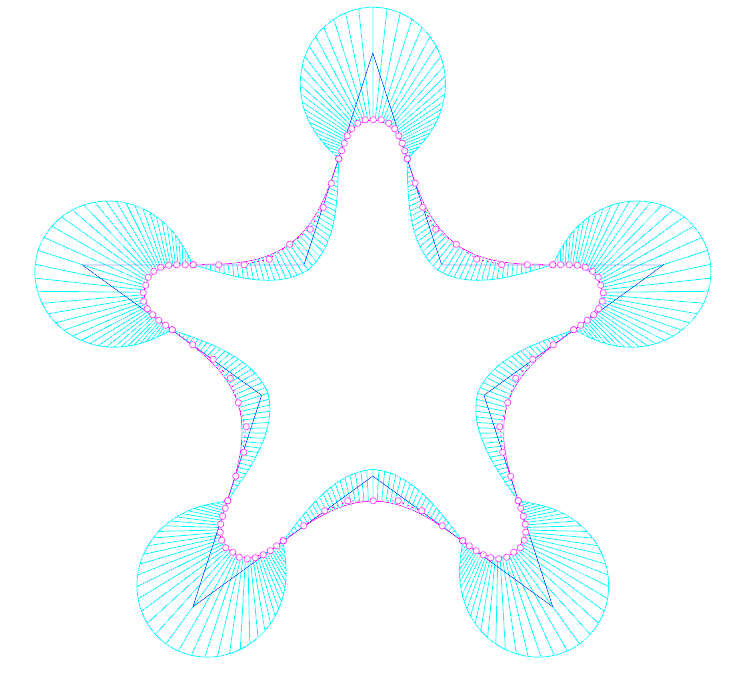
\includegraphics[width=0.9\linewidth]{figures/SmoothingCorner3.png}
		\end{minipage}
		%\qquad
		\begin{minipage}{0.49\linewidth}
			\centering
			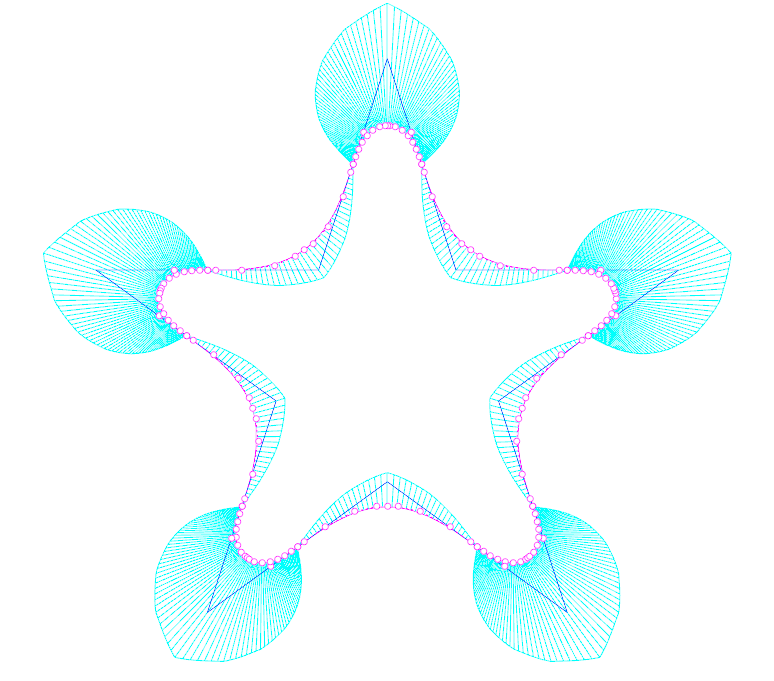
\includegraphics[width=0.9\linewidth]{figures/SmoothingCorner4.png}
		\end{minipage}
	
		\caption{\small{对正五角星的每一个角做圆角, 圆角的起点和终点均为各边中点. 左图: 使用Euler B\'ezier曲线生成, 钝角的圆角曲线是两段4次曲线, 锐角的圆角为两段7次曲线. 右图: 使用Euler B-Spline曲线生成, 所有曲线均为三次. 两个例子都表现出了$G^2$连续性, B\'ezier曲线次数更高, 每一段内的几何连续性也更高, B-Spline曲线次数恒定, 但由于拼接, 几何连续性只能达到$G^2$.}}
		\label{pentagram}
	\end{figure}
\begin{figure}
	\centering
	\begin{minipage}{0.49\linewidth}
		\centering
		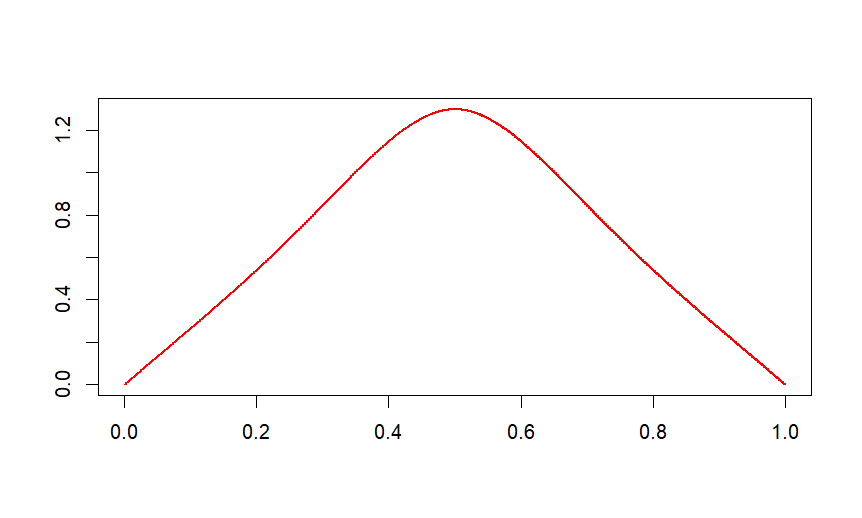
\includegraphics[width=0.7\linewidth]{figures/Pentagram_Bezier1.png}
	\end{minipage}
	%\qquad
	\begin{minipage}{0.49\linewidth}
		\centering
		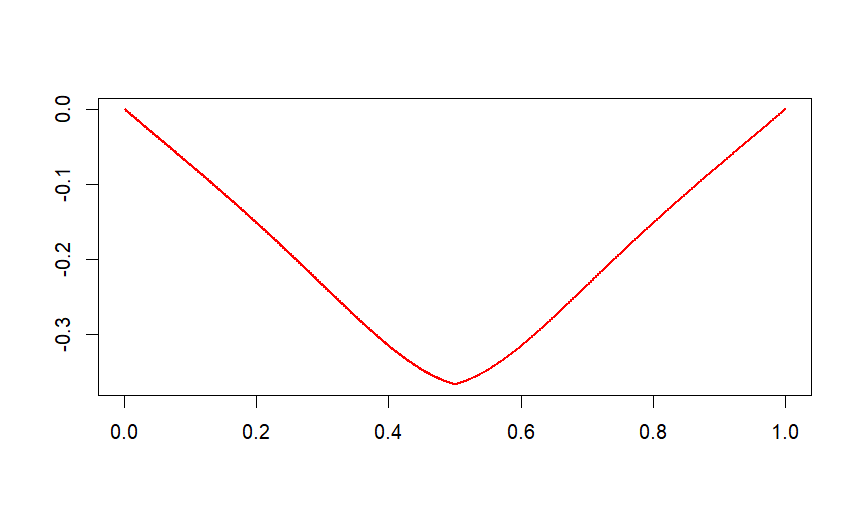
\includegraphics[width=0.7\linewidth]{figures/Pentagram_Bezier2.png}
	\end{minipage}
\caption{\small{图(\ref{pentagram})中两个B\'ezier圆角的曲率}}
\end{figure}
\begin{figure}
	\centering
	\begin{minipage}{0.49\linewidth}
		\centering
		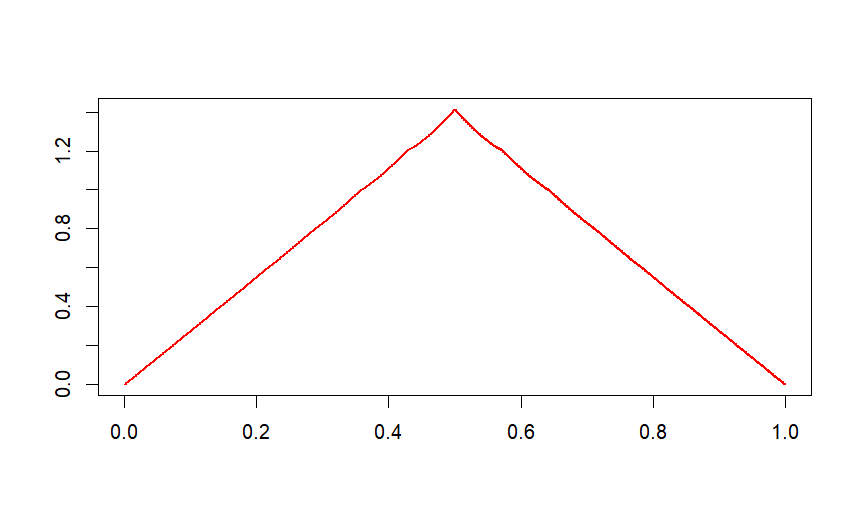
\includegraphics[width=0.7\linewidth]{figures/Pentagram_B-Spline1.png}
	\end{minipage}
	%\qquad
	\begin{minipage}{0.49\linewidth}
		\centering
		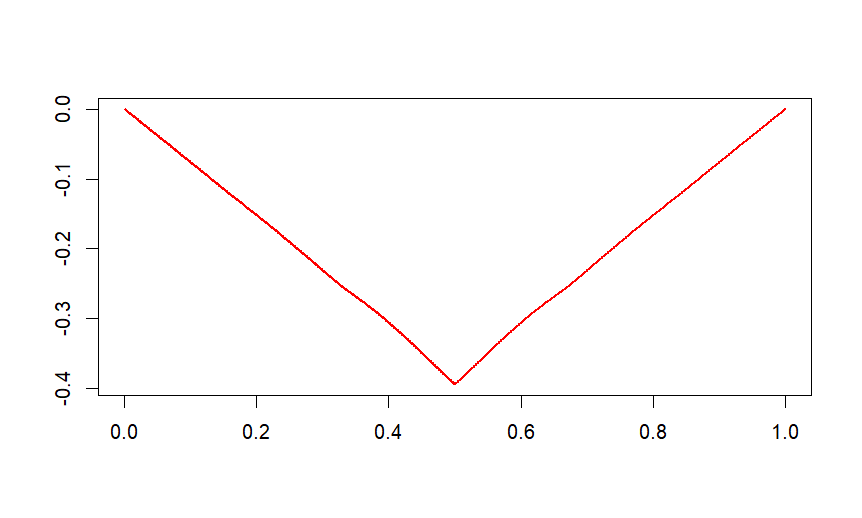
\includegraphics[width=0.7\linewidth]{figures/Pentagram_B-Spline2.png}
	\end{minipage}
\caption{\small{图(\ref{pentagram})中两个B-Spline圆角的曲率}}
\end{figure}
	 \section{空间Euler B\'{e}zier 曲线与Euler B-Spline 曲线}
	 \subsection{空间Euler螺线}
	 平面的各种螺线很早以前就有各种定义和性质的研究, 一般而言可以概括为曲率$\kappa(s)^{\alpha} = as+b$, 即曲率的某个方幂与弧长是线性关系,$\alpha=1$为Euler螺线, $\alpha=-1$是对数螺线, $\alpha=-2$为圆的渐开线, 这样的曲线其显著特征就是曲率的单调性. 在空间中对于螺线的定义应该同时包括曲率和挠率, 我们采用Euler螺线定义方法, 将曲率$\kappa$, 挠率$\tau$均与弧长呈线性关系, 
	  \begin{definition}[空间Euler螺线]
	 	设$\boldsymbol{P}(t), t\in[t_0,t_1]$是空间中的一段曲线, 设$s$为其弧长参数, 如果其曲率$\kappa(s)$和挠率$\tau(s)$ 满足$\kappa(s) = as+b,\quad\tau(s) = cs+d$, 其中$a,b,c,d$均是常数, 则称$\boldsymbol{P}(t)$是空间Euler螺线.
	 \end{definition}
	 事实上, 根据曲线论的第一基本定理可知, 给定了常数$a,b,c,d$后, 这样定义的空间Euler螺线一定存在, 并且在相差一个刚体运动的意义下是唯一的. 不过, 直接试图求解这样的曲线并不是好的选择, 一方面它需要求解Frenet微分方程组得到离散结果, 不能得到准确的参数化表示, 更不能表示成NURBS曲线; 另一方面是实际应用中往往要构造满足$G^1$边值条件的曲线, 在这种情况下这样严格定义的曲线未必是存在的. 所以我们将空间Euler螺线的几何性质离散化, 计算出一个可以逼近Euler螺线的离散多边形, 再利用B样条曲线或B\'ezier曲线能逼近多边形控制顶点的性质, 来构造能准确参数化的多项式曲线. 因此我们和平面有类似的方法, 引入空间Euler多边形.
	
	 \subsection{空间Euler多边形}
	 三维空间中插值$G^1$边界条件的曲率(以及挠率)单调曲线的存在性不像二维的情形有简单且完整的理论证明. 现有的一些构造三维螺线的结果有对于离散多边形的非线性细分方法, 有根据Frenet方程的离散形式进行计算的方法, 这些方法得到的都是离散形式的曲线, 需要进行多次迭代, 或者计算大量的采样点, 而我们的目的是使用显式的(分段)多项式曲线来尽可能的构造曲率单调曲线. 将空间Euler螺线按弧长参数均匀采样点会得到一个多边形, 我们可以去在多边形中寻找一些离散的量作为曲线曲率和挠率连续量的近似. 曲率反映了切向的变化速度, 因此我们可以用边之间的角度大小来衡量曲率的大小, 但是不同于二维情况, 三维的曲率是没有正负号, 即曲率向量的方向可以是任意的, 但是角度的大小不能体现这一点, 所以我们把空间的Euler多边形看作平面的Euler多边形“扭曲”得到的. 我们使用多边形相邻边的两种角度来反映曲率和挠率, 一种是将两条边投影到xOy平面上, 投影后两向量的符号角度, 定义为“水平角度”; 另一种是两条边的俯仰角的差值, 定义为“竖直角”, 参见图(\ref{explain})\par 
	 \begin{figure}[ht]
	 	\centering
	 	
	 	\begin{minipage}[b]{0.33\textwidth} % 左半部分
	 		\centering
	 		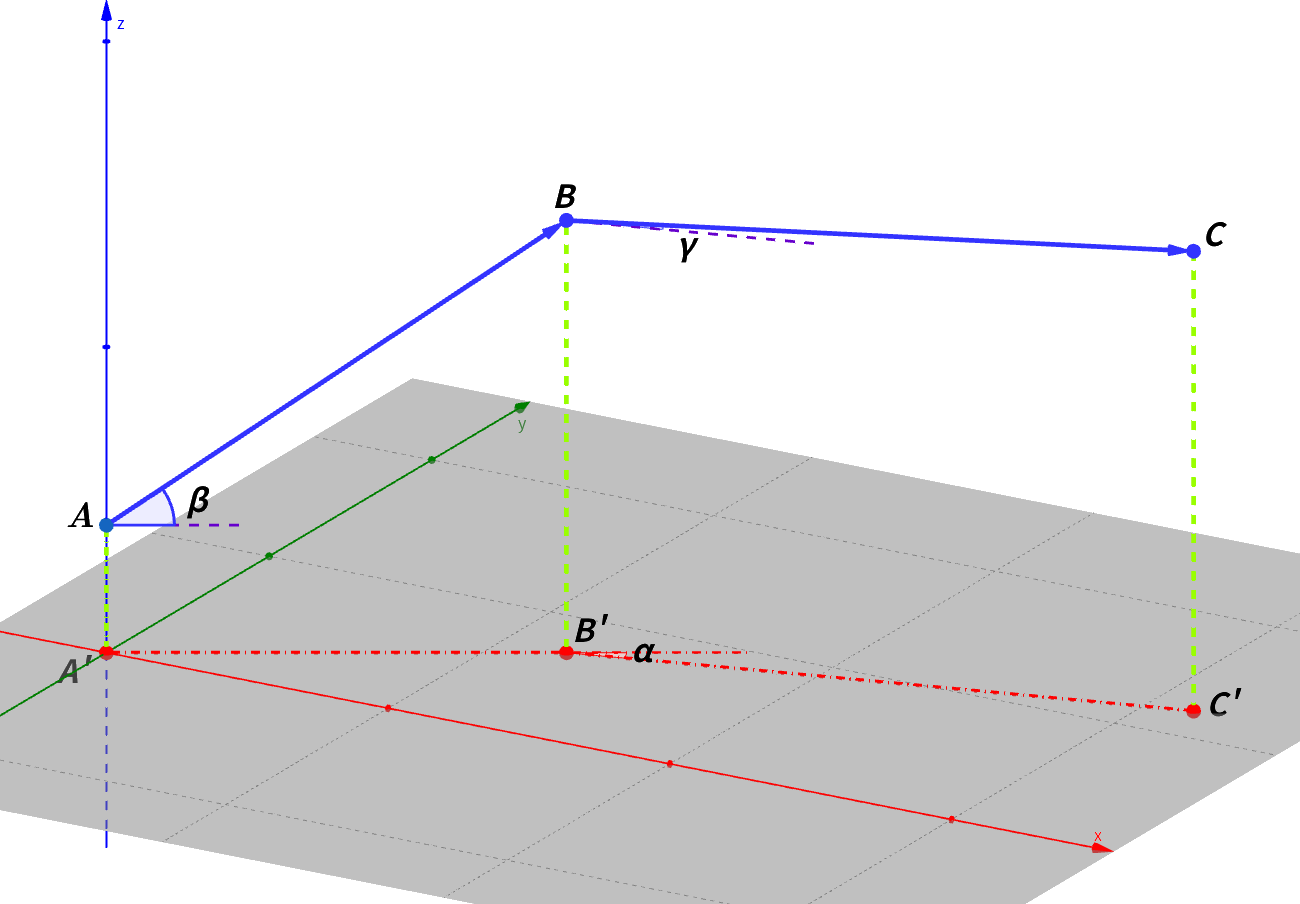
\includegraphics[width=\textwidth]{figures/explain_angle_main.png}
	 	\end{minipage}\hfill
	 	\begin{minipage}[b]{0.33\textwidth} % 右半部分
	 		\centering
	 		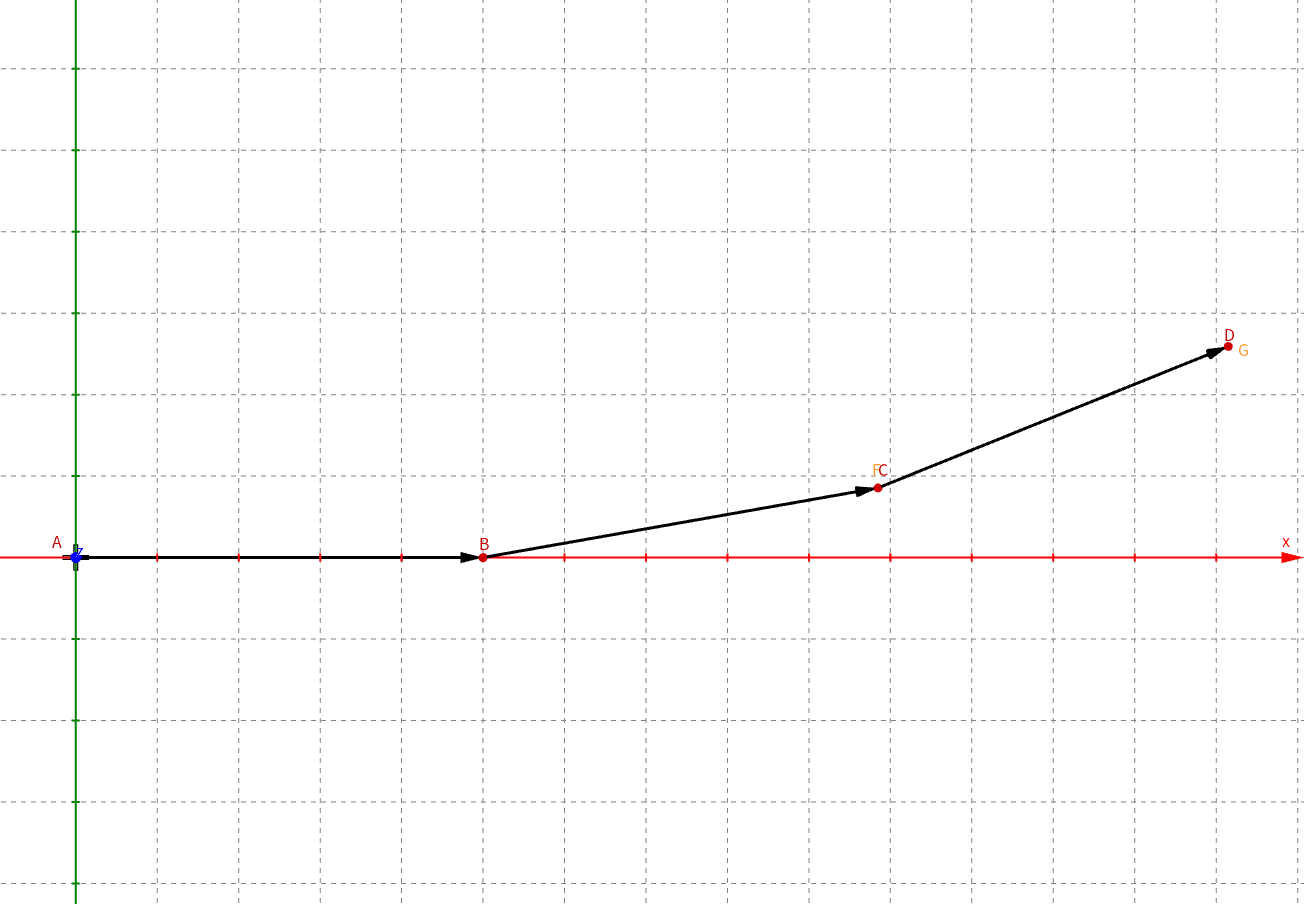
\includegraphics[width=\textwidth]{figures/explain_angle_top.png}
	 	\end{minipage}
 	\begin{minipage}[b]{0.33\textwidth} % 右半部分
 		\centering
 		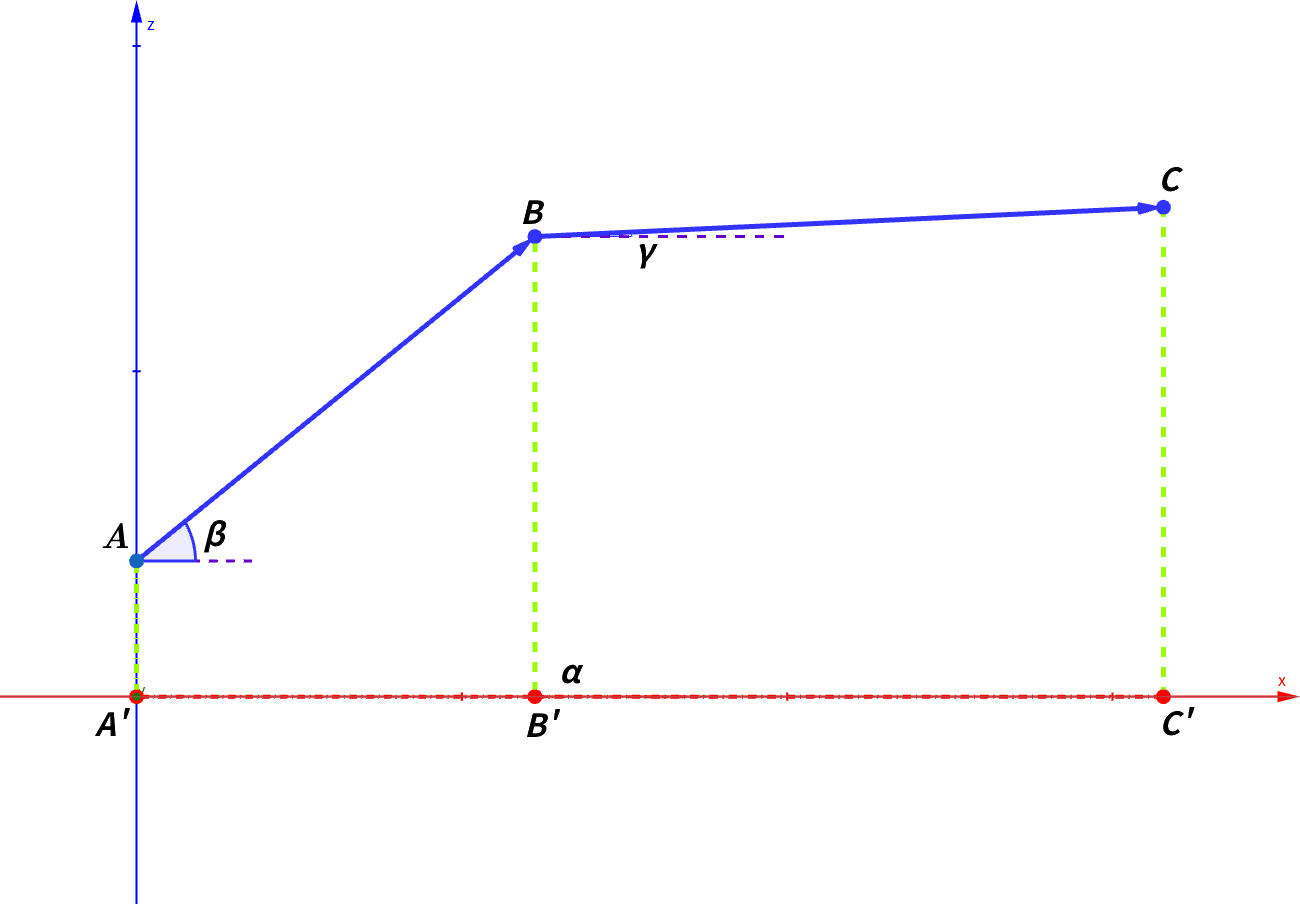
\includegraphics[width=\textwidth]{figures/explain_angle_front.png}
 	\end{minipage}

	 	\caption{\small{左, 中, 右分别是一段空间多边形角点$\boldsymbol{ABC}$的标准视图, 顶视图和主视图,  $\boldsymbol{A}'$,$\boldsymbol{B}'$,$\boldsymbol{C}'$分别为三点在xOy平面的投影. $\boldsymbol{A}'\boldsymbol{B}'$与$\boldsymbol{B}'\boldsymbol{C}'$的夹角$\alpha$定义为多边形角点$\boldsymbol{B}$的水平角$\theta_{\boldsymbol{B}}$. $\beta$和$\gamma$分别是向量$\boldsymbol{AB}$, $\boldsymbol{BC}$与xOy平面的夹角, 我们定义点$\boldsymbol{B}$处的竖直角$\phi_{\boldsymbol{B}}=\gamma-\beta$. }}
	 	 \label{explain}
	 \end{figure}
	  下面给出两种角的严格定义. 假设有非零的三维向量$\boldsymbol{v}=(v_x,v_y,v_z)$, 将其化为极坐标得到$\hat{\boldsymbol{v}}=(\rho_v,\theta_v,\phi_v)$, 其中$\rho_v>0$是$\boldsymbol{v}$的模长, $\theta_v\in[0,2\pi)$是$\boldsymbol{v}$在xy平面投影向量的极角, $\phi_v\in[-\frac{\pi}2,\frac{\pi}2]$是$\boldsymbol{v}$的仰角, 它们满足等式
	 \begin{equation}\label{angle_compute}
	 \begin{aligned}
	 &\rho_v = \sqrt{v_x^2+v_y^2+v_z^2}\\
	 &\theta_v =
	 \left\{
	 \begin{aligned}
	 &\arccos(\frac{v_x}{\sqrt{v_x^2+v_y^2}}),\quad &v_x^2+v_y^2>0, v_y\geq0\\
	 &-\arccos(\frac{v_x}{\sqrt{v_x^2+v_y^2}})+2\pi, \quad &v_x^2+v_y^2>0, v_y<0\\
	 &0, \quad &v_x=v_y=0
	 \end{aligned}
	 \right.\\
	 &\phi_v = \left\{
	 \begin{aligned}
	 &\arctan(\frac{v_z}{\sqrt{v_x^2+v_y^2}}),\quad &v_x^2+v_y^2>0\\
	 &\mathrm{sign}(v_z)*\frac{\pi}2,\quad &v_x=v_y=0
	 \end{aligned}
	 \right.
	 \end{aligned}
	 \end{equation} 对于一个空间多边形$\boldsymbol{P}_0,\dots,\boldsymbol{P}_n$, 它的n条边$\boldsymbol{P}_i\boldsymbol{P}_{i+1}$记为向量$\boldsymbol{v}_i(0\leq i\leq n-1)$, 其极坐标表示的极角和俯角记为$\theta_{v_i}, \phi_{v_i}$, 记相邻边$\boldsymbol{v}_i, \boldsymbol{v}_{i+1}$的水平夹角为$\theta_i = \theta_{v_{i+1}}-\theta_{v_i}$, 相邻边$\boldsymbol{v}_i, \boldsymbol{v}_{i+1}$的竖直夹角为$\phi_i = \phi_{v_{i+1}}-\phi_{v_i}$, $0\leq i\leq n-2$我们使用这两种角定义三维的Euler多边形.
	 \begin{definition}[空间Euler多边形]\label{EP3D_Def}
	 	
	 	设三维空间中有多边形$\boldsymbol{P}_0,\dots,\boldsymbol{P}_n$, 顶点互不相同, 如果它们的相邻边的水平夹角$\theta_i$, 竖直夹角$\phi_i$满足:
	 	\begin{equation}
	 		\begin{aligned}
	 		(1).\quad &\theta_i-2\theta_{i+1}+\theta_{i+2} = 0,\quad i=0,1,\dots,n-4\\
	 		(2).\quad &\phi_i-2\phi_{i+1}+\phi_{i+2} = 0,\quad i=0,1,\dots,n-4\\
	 		(3).\quad &\text{所有边长}\Arrowvert\boldsymbol{v_i}\Arrowvert\text{相等} 
	 		\end{aligned}
	 	\end{equation}
	 	则称$\boldsymbol{P}_0,\dots,\boldsymbol{P}_n$是三维Euler多边形.
	 \end{definition}
	 由空间Euler多边形作为控制顶点生成的B\'ezier曲线或整数节点B样条曲线称为空间Euler B\'ezier曲线或空间Euler B-Spline曲线. \par 
	 假定有三维$G^1$条件: 起点$\boldsymbol{P}_S$, 终点$\boldsymbol{P}_E$, 以及起点终点切向$\boldsymbol{T}_S$, $\boldsymbol{T}_E$, 其中$\boldsymbol{T}_S$, $\boldsymbol{T}_E$是单位向量, 并且与起点指向终点的向量$\boldsymbol{P}_S\boldsymbol{P}_E$, 三个向量异面. 对于这样的$G^1$条件, 直接构造严格满足定义(\ref{EP3D_Def})的曲线是行不通的, 事实上在二维情况下都是不可行的, 所以我们依然使用一种非线性细分的方法对初始多边形进行迭代, 使其逐渐逼近三维的Euler多边形, 当然没有理论保证对于任意的边值条件都存在满足定义(\ref{EP3D_Def})的多边形, 但是如果这样的多边形存在, 我们的方法可以很好的逼近出这样的多边形, 以它们作为控制顶点的B\'ezier和B-Spline曲线是曲率单调的.
	 \subsection{空间Euler B\'{e}zier 曲线}
	 对于一般的三维$G^1$边值条件, 我们先作刚体变换使得起点$\boldsymbol{P}_S$位于原点, 初始切向变换为x轴正向的单位向量$(1,0,0)$并且终点的端切向与xOy平面平行, 这样的变换是非常容易的, 只需要一次平移和旋转即可. \par
	 变换后的边值条件, 起点和起点端切向即为$\boldsymbol{P}_S=(0,0,0), \boldsymbol{T}_S = (1,0,0)$, 终点的端切向与xOy平面平行. 我们很容易构造一个初始多边形, 使得该多边形生成的B\`ezier曲线满足该$G^1$边值条件, 这样的多边形至少要四个顶点, 可以表示为
	 \begin{equation}
	 	\begin{aligned}
	 		&\boldsymbol{P}_0 = \boldsymbol{P}_S\\
	 		&\boldsymbol{P}_1 = \boldsymbol{P}_S+\lambda\boldsymbol{T}_S\\
	 		&\boldsymbol{P}_2 = \boldsymbol{P}_E-\mu\boldsymbol{T}_E\\
	 		&\boldsymbol{P}_3 = \boldsymbol{P}_E
	 	\end{aligned}
	 \end{equation}
	 其中$\lambda, \mu>0$是可变的常数, 我们可以选择设置为$\lambda = \mu = \Arrowvert\boldsymbol{P}_S\boldsymbol{P}_E\Arrowvert/3$. \par 
	 接下来, 我们从初始多边形开始进行保边界条件的迭代. 假设当前的多边形顶点按顺序为$\boldsymbol{P}_0, \dots,\boldsymbol{P}_n$, 那么$\boldsymbol{P}_0$和$\boldsymbol{P}_n$的位置不变, $\boldsymbol{P}_1$和$\boldsymbol{P}_{n-1}$的位置只依赖于多边形的边长, 因为它们用于满足端切向条件, 所以从$\boldsymbol{P}_2$开始计算. 假定现有连续的三点$\boldsymbol{P}_{i-1},\boldsymbol{P}_i,\boldsymbol{P}_{i+1}$, 其中$i=2,\dots,n-2$, 我们计算新的$\hat{\boldsymbol{P}}_i$更新该多边形. 我们把多边形相交于顶点$\boldsymbol{P}_i$的边$\boldsymbol{v}_{i-1}$和$\boldsymbol{v}_{i}$的水平, 竖直夹角称为点$\boldsymbol{P}_i$处的水平, 竖直转角, 记为$\theta_i$和$\phi_i$(定义(\ref{EP3D_Def})). 为了在局部满足Euler多边形的条件, 应当让转角满足$2\theta_i = \theta_{i-1}+\theta_{i+1}$, 以及$2\phi_{i} = \phi_{i-1}+\phi_{i+1}$, 因此, 我们更新$\boldsymbol{P}_i$处的转角为:
	 \begin{equation}\label{new_theta}
	 	\begin{aligned}
	 		&\hat{\theta}_i = \frac{\theta_{i-1}+\theta_i+\theta_{i+1}}3\\
	 		&\hat{\phi}_i =
	 		\frac{\phi_{i-1}+\phi_i+\phi_{i+1}}3
	 	\end{aligned}
	 \end{equation}
	 接下来, 我们通过已经更新的$\hat{\theta}_i$和$\hat{\phi}_i$来确定$\hat{\boldsymbol{P}}_i$的位置. 设$\boldsymbol{P}_{i-1}$和$\boldsymbol{P}_{i+1}$的坐标分别为$(x_1,y_1,z_1)$和$(x_2,y_2,z_2)$, $\boldsymbol{P}_{i-1}$和$\boldsymbol{P}_{i+1}$在xOy平面上的投影记为$\bar{\boldsymbol{P}}_{i-1}$和$\bar{\boldsymbol{P}}_{i+1}$, 所求的新$\hat{\boldsymbol{P}}_i$在xOy面上的投影为$\bar{\hat{\boldsymbol{P}}}_i$. 我们要使得$\bar{\boldsymbol{P}}_{i-1}$, $\bar{\hat{\boldsymbol{P}}}_i$和$\bar{\boldsymbol{P}}_{i+1}$三点形成的转角为$\hat{\theta}_i$, 从而点$\bar{\hat{\boldsymbol{P}}}_i$应当位于一段圆弧上, 该圆弧的半径为
	 \begin{equation}\label{R}
	 R = \frac{\Arrowvert\bar{\boldsymbol{P}}_{i-1}\bar{\boldsymbol{P}}_{i+1}\Arrowvert}{2\sin(\hat{\theta}_i)}
	 \end{equation}
	 圆心的位置也可以由下式给出
	 \begin{equation}\label{center}
	 C_i = \frac{\bar{\boldsymbol{P}}_{i-1}+\bar{\boldsymbol{P}}_{i+1}}2+\mathrm{R}(\mathrm{sign}(\hat{\theta}_i)\cdot\frac{\pi}2)\cdot\frac{\bar{\boldsymbol{P}}_{i-1}\bar{\boldsymbol{P}}_{i+1}}{\Arrowvert\bar{\boldsymbol{P}}_{i-1}\bar{\boldsymbol{P}}_{i+1}\Arrowvert}\cdot\sqrt{R^2-\frac14\Arrowvert\bar{\boldsymbol{P}}_{i-1}\bar{\boldsymbol{P}}_{i+1}\Arrowvert^2}
	 \end{equation}
	 其中$\mathrm{R}(\theta)$表示在xOy平面绕原点旋转$\theta$角度, 注意到$\hat{\theta}_i$是有符号的, 并且圆心与点$\bar{\hat{\boldsymbol{P}}}_i$位于$\bar{\boldsymbol{P}}_{i-1}\bar{\boldsymbol{P}}_{i+1}$的两侧. 将$C_i$的坐标记为$(a,b)$, 从而我们可以设$\bar{\hat{\boldsymbol{P}}}_i=(a+R\cos(x),b+R\sin(x))$, 设$\hat{\boldsymbol{P}}_i=(a+R\cos(x),b+R\sin(x),z)$. \par 
	 接下来考虑竖直角, 向量$\boldsymbol{P}_{i-1}\hat{\boldsymbol{P}}_i$和$\hat{\boldsymbol{P}}_i\boldsymbol{P}_{i+1}$的俯角应当满足
	 \begin{equation}
	 \begin{aligned}
	 &\tan(\phi_{\boldsymbol{P}_{i-1}\hat{\boldsymbol{P}}_i}) = \frac{z-z_1}{\boldmath{L}_1(x)}\\
	 &\tan(\phi_{\hat{\boldsymbol{P}}_i\boldsymbol{P}_{i+1}}) = \frac{z_2-z}{\boldmath{L}_2(x)}
	 \end{aligned}
	 \end{equation}
	 其中, $\boldmath{L}_1(x)$和$\boldmath{L}_2(x)$分别表示点$\bar{\hat{\boldsymbol{P}}}_i$到点$\bar{\boldsymbol{P}}_{i-1}$和点$\bar{\boldsymbol{P}}_{i+1}$的距离.
	 
	 \begin{figure}[ht]
	 	\centering
	 
	 	\begin{minipage}[b]{0.45\textwidth} % 
	 		\centering
	 		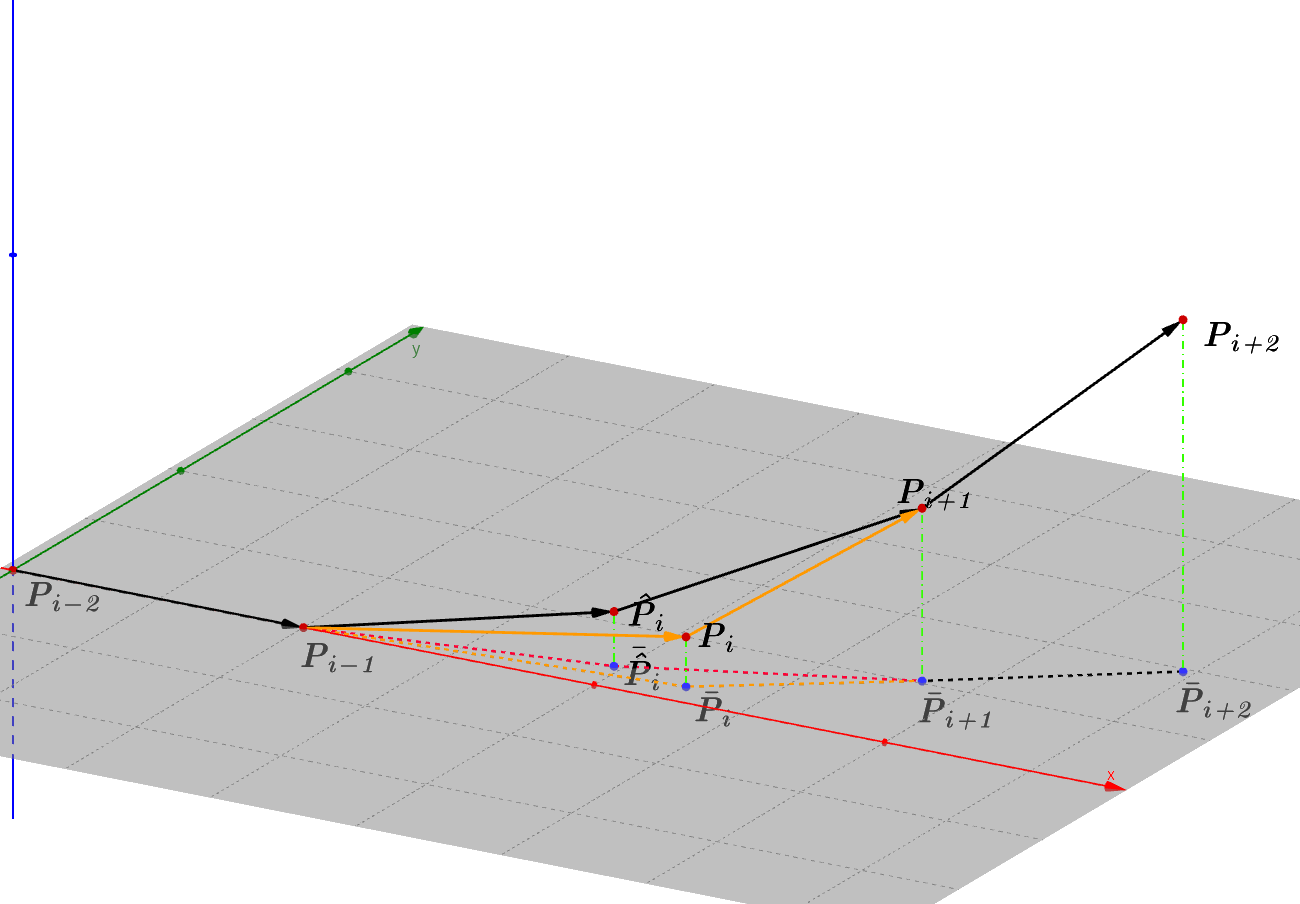
\includegraphics[width=\textwidth]{figures/al_main_bold.png}
	 	\end{minipage}\hfill
	 	\begin{minipage}[b]{0.45\textwidth} % 
	 		\centering
	 		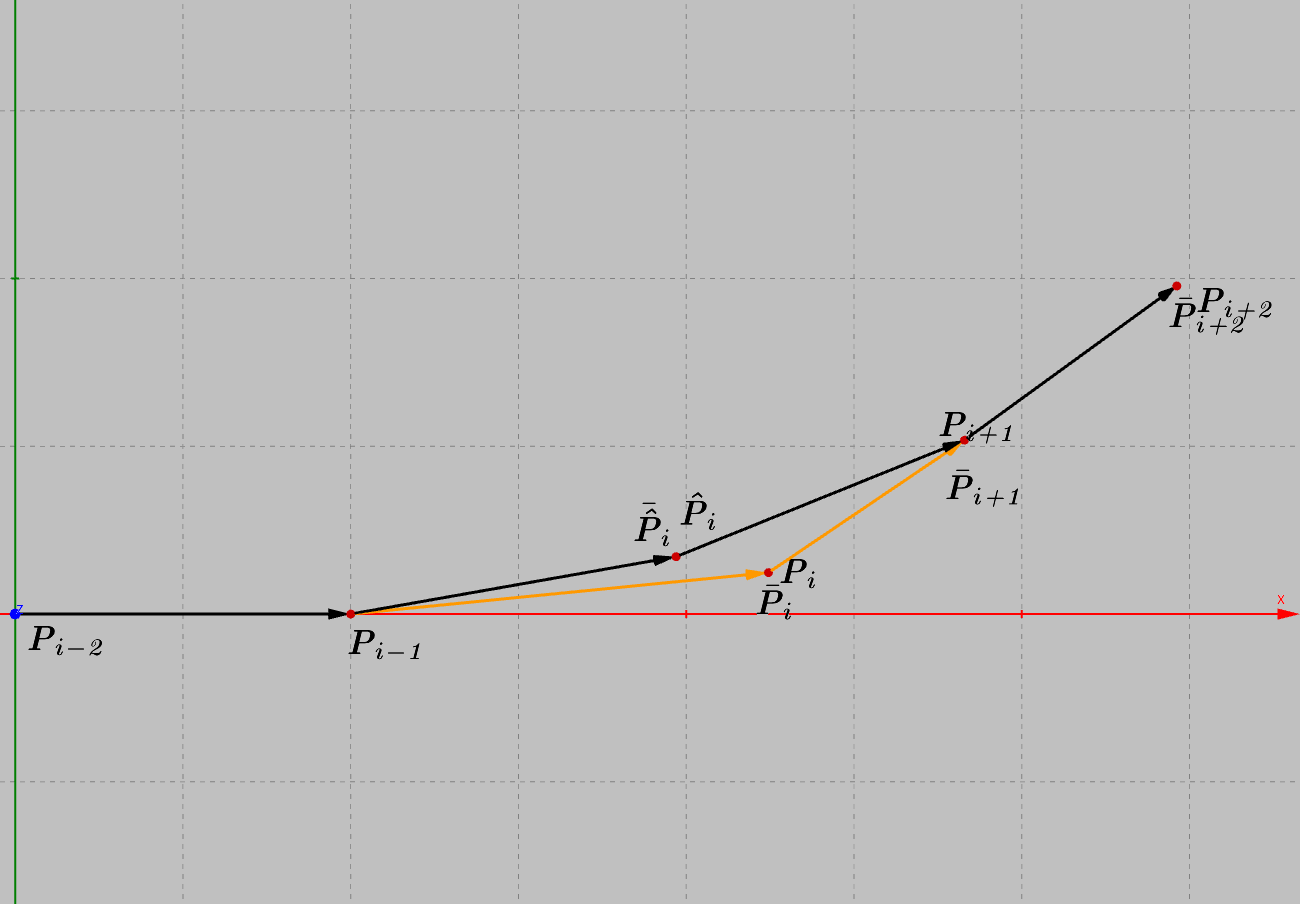
\includegraphics[width=\textwidth]{figures/al_top_bold.png}
	 	\end{minipage}
	 	\caption{算法图解. }
	 	\label{algorithm_explain}
	 \end{figure}
	 
	 
	  我们要使$\phi_{\hat{\boldsymbol{P}}_i\boldsymbol{P}_{i+1}}-\phi_{\boldsymbol{P}_{i-1}\hat{\boldsymbol{P}}_i}=\hat{\phi_i}$, 从而得到方程
	 \begin{equation}\label{eq1}
	 \frac{z_2-z}{\boldmath{L}_2(x)}-\frac{z-z_1}{\boldmath{L}_1(x)} = \tan(\hat{\phi_i})(1+\frac{(z_2-z)(z-z_1)}{\boldmath{L}_1(x)\boldmath{L}_2(x)})
	 \end{equation}
	 最后再利用Euler多边形的各边相等, 要有$\Arrowvert\boldsymbol{P}_{i-1}\hat{\boldsymbol{P}}_i\Arrowvert = \Arrowvert\boldsymbol{P}_{i+1}\hat{\boldsymbol{P}}_i\Arrowvert$, 则有方程
	 \begin{equation}\label{eq2}
	 \boldmath{L}_1(x)^2+(z-z_1)^2 =\boldmath{L}_2(x)^2+(z_2-z)^2
	 \end{equation}
	 注意到式(\ref{eq2})等价于
	 \begin{equation}
	 z = \frac{z_1+z_2}2+\frac{\boldmath{L}_1(x)^2-\boldmath{L}_2(x)^2}{2(z_1-z_2)}
	 \end{equation}
	 将其代入式(\ref{eq1}), 并记$z_2-z_1 = h$得到
	 \begin{equation}\label{eq_final}
	 \begin{aligned}
	 \boldmath{L}_1(x)(\frac h2+\frac{\boldmath{L}_1(x)^2-\boldmath{L}_2(x)^2}{2h})-\boldmath{L}_2(x)(\frac h2-\frac{\boldmath{L}_1(x)^2-\boldmath{L}_2(x)^2}{2h})\\
	 -\tan(\hat{\phi_i})(\boldmath{L}_1(x)\boldmath{L}_2(x)+\frac{h^2}4-\frac{(\boldmath{L}_1(x)^2-\boldmath{L}_2(x)^2)^2}{4h^2})=0
	 \end{aligned}
	 \end{equation}
	 将式(\ref{eq_final})左侧的表达式记为$\Phi(x)$, 我们即要求$\Phi(x)$的零点. \par 
	 关于函数$\Phi(x)$的零点, 我们可以证明在一定条件下零点是存在的(但是不一定唯一), 我们令$L$表示点$\bar{\boldsymbol{P}}_{i-1}$到点$\bar{\boldsymbol{P}}_{i+1}$的距离, 我们注意到当点$\bar{\hat{\boldsymbol{P}}}_i$与$\bar{\boldsymbol{P}}_{i-1}$重合时, $\boldmath{L}_1(x)$的值为0, $\boldmath{L}_2(x)$的值为$L$, 将此时的$x$的值记为$x_1$; 同理记另一端极限情况的$x$的值为$x_2$, 满足$\boldmath{L}_1(x_2)=L, \boldmath{L}_2(x_2)=0$, 不妨假设$x_1<x_2$. 我们可以得到一个使解存在的充分条件
	 \begin{theorem}
	 	若$|h|<L$, 则关于$x$的方程(\ref{eq_final})在区间$[x_1,x_2]$上一定有解. 
	 \end{theorem}
{\indent\bf 证明} \par 考虑函数$\Phi(x)$在区间端点和中点处的取值, 我们有
\begin{equation}
\begin{aligned}
&\Phi(x_1) = \frac{h^2+L^2}4[\tan(\hat{\phi}_i)(\frac Lh)^2-2(\frac Lh)-\tan(\hat{\phi}_i)]\\
&\Phi(x_2) = \frac{h^2+L^2}4[\tan(\hat{\phi}_i)(\frac Lh)^2+2(\frac Lh)-\tan(\hat{\phi}_i)]\\
&\Phi(x_0) = -\tan(\hat{\phi}_i)(L_0^2+\frac{h^2}4)
\end{aligned}
\end{equation}
其中$x_0 = \frac{x_1+x_2}2$, 根据几何性质显然有$\boldmath{L}_1(x_0) = \boldmath{L}_2(x_0)$, $L_0$表示这一对相等的长度. \par 
我们不妨假设$\hat{\phi}_i\in(0,\frac{\pi}2)$, 记函数$\boldmath{F}_1(x) = \tan(\hat{\phi}_i)x^2-2x-\tan(\hat{\phi}_i)$, $\boldmath{F}_2(x) = \tan(\hat{\phi}_i)x^2+2x-\tan(\hat{\phi}_i)$, 两个函数的图像如图(\ref{f1f2}), 
\begin{figure}[h]
	\centering
	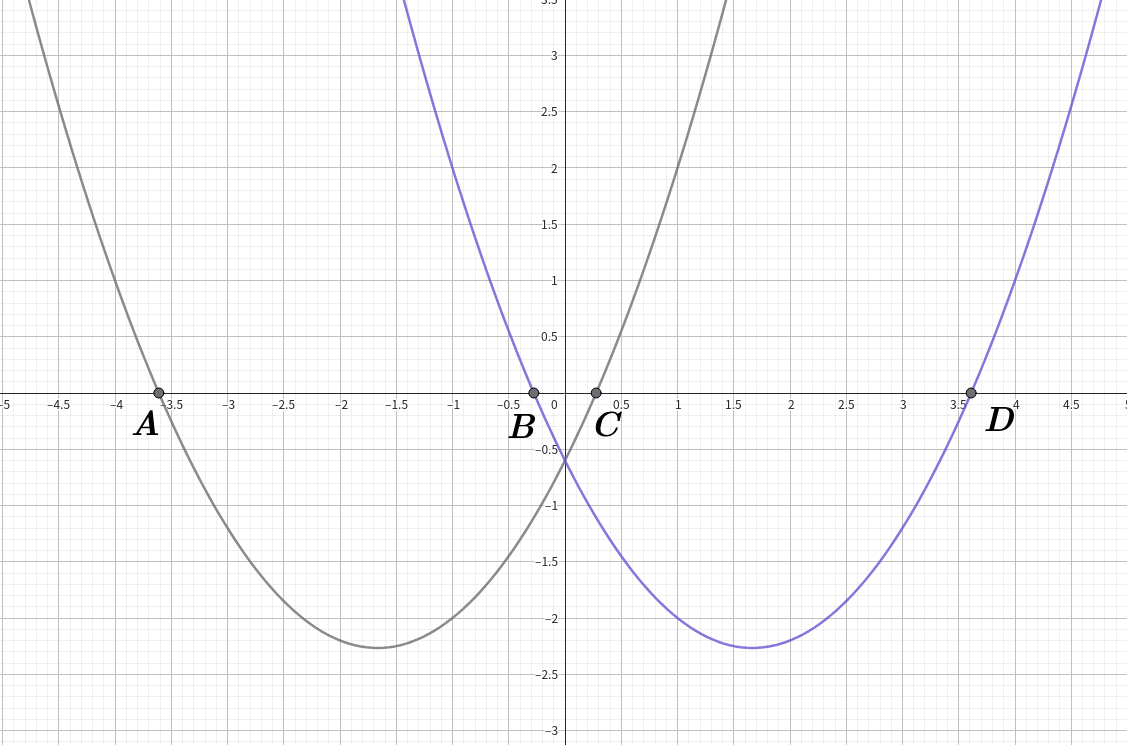
\includegraphics[width = 0.6\textwidth]{figures/f1f2.png}
	\label{f1f2}
\end{figure}
 两函数共有四个零点, 我们可以求得它们从小到大分别为$$-\frac{1}{\tan(\frac{\hat{\phi}_i}2)}, -\tan(\frac{\hat{\phi}_i}2),\tan(\frac{\hat{\phi}_i}2),\frac 1{\tan(\frac{\hat{\phi}_i}2)}. $$
 如果$L/h$的值在图中$AB$或$CD$之间, 即若$\tan(\frac{\hat{\phi}_i}2)<|L/h|<\frac 1{\tan(\frac{\hat{\phi}_i}2)}$, 则$\Phi(x_1)\Phi(x_2)<0$, 那么方程(\ref{eq_final})显然有解. 如果$|L/h|> 1/\tan(\frac{\hat{\phi}_i}2)$, 那么$\Phi(x_1), \Phi(x_2)>0$, 而$\Phi(x_0)<0$, 从而方程(\ref{eq_final})仍然有解. 也就是说, 只要$|L/h|>\tan(\frac{\hat{\phi}_i}2)$, 解就一定存在, 由于我们可以细分多边形使得$\hat{\phi}_i<\pi/2$, 从而$\tan({\hat{\phi}_i}/2)<1$, 结论成立.
 $\square$\par 
	 求得了满足条件的$x$后, 可以代入求得$\hat{\boldsymbol{P}}_i$的坐标, 用新坐标更新顶点序列的$\boldsymbol{P}_i$, 之后对于下一个顶点重复上述步骤. 最后计算$\boldsymbol{P}_1, \boldsymbol{P}_{n-1}$的值, 我们计算当前多边形的平均边长$\bar{L}$, 令$\boldsymbol{P}_1 = \boldsymbol{P}_0+\bar{L}\boldsymbol{T}_S$, $\boldsymbol{P}_{n-1} = \boldsymbol{P}_n-\bar{L}\boldsymbol{T}_E$计算出所有顶点. \par 
	 每当对所有顶点完成一次迭代, 我们计算当前的角度误差量
	 \begin{equation}\label{error}
	 \begin{aligned}
	 &E_{\theta} = \max_{2\leq i\leq n-2}|2\theta_i-\theta_{i-1}-\theta_{i+1}|\\
	 &E_{\phi} = \max_{2\leq i\leq n-2}|2\phi_i-\phi_{i-1}-\phi_{i+1}|
	 \end{aligned}
	 \end{equation}
	 以及所有边长长度的标准差$\sigma_L$, 为这三个量分别设定阈值, 不断迭代直到三个量均小于阈值, 此时可以认为多边形是近似的Euler多边形. 迭代的过程中顶点数是不会增加的, 我们在每一次迭代至满足要求后对多边形升阶, 再迭代得到更逼近的结果, 升阶的方法为
	 \begin{equation}
	 \hat{\boldsymbol{P}}_i = \boldsymbol{P}_{i-1}\cdot\frac{i}{n+1}+\boldsymbol{P}_{i}\cdot(1-\frac{i}{n+1}), i=0,1,\dots,n+1
	 \end{equation}
	 经过迭代和升阶, 最终可以得到满足要求的曲线, 该算法的伪代码表示见算法(\ref{smoothcurve3})
	 \IncMargin{1em}
	 \begin{algorithm}
	 	\SetKwData{Left}{left}\SetKwData{This}{this}\SetKwData{Up}{up}
	 	\SetKwFunction{Union}{Union}\SetKwFunction{FindCompress}{FindCompress}
	 	\SetKwInOut{Input}{input}\SetKwInOut{Output}{output}
	 	\caption{3D Euler B\'{e}zier 曲线}\label{smoothcurve3}
	 	\KwData{初始的三维控制多边形$\boldsymbol{P}_0\dots\boldsymbol{P}_m$, 最大迭代次数$\mathrm{max\_n}$. }
	 	\KwResult{
	 		与初始曲线有相同$G^1$边值条件的Euler B\'ezier曲线. }
	 	\BlankLine 
	 	$n=m-1$\;
	 	求旋转矩阵$\boldmath{R}$, 使旋转后的两端切向与xOy平面平行\;
	 	将旋转后的多边形重新记为$\boldsymbol{P}_0\dots\boldsymbol{P}_m$, 用$\boldsymbol{T}_S, \boldsymbol{T}_E$表示起终点单位切向\;
	 	声明两个角度序列AngleTheta[n], AnglePhi[n]\;
	 	AngleTheta[0]=0.0, AngleTheta[n-1]=0.0\;
	 	AnglePhi[0]=0.0, AnglePhi[n-1]=0.0\;
	 	\For{$\mathrm{(i=1;i<n-1;i=i+1)}
	 		$}
	 	{根据式(\ref{angle_compute})计算AngleTheta[i], AnglePhi[i]\;}
	 	\While{$\mathrm{(n<=max_n)}$}{
	 		E\_theta = 10.0, E\_phi = 10.0, sigma\_L = 10.0\;
	 		s\_count = 1\;
	 		max\_count = 10000\;
	 		\While{$\mathrm{(s\_count<max\_count \&\& (E\_theta>1e-6 || E\_phi>1e-6 || sigma\_L>1e-6))}$}{\For{$\mathrm{(i=2;i<n-2;i=i+1)}
	 				$}{AngleTheta[i] = (AngleTheta[i-1]+AngleTheta[i]+AngleTheta[i+1])/3\;
	 				AnglePhi[i] = (AnglePhi[i-1]+AnglePhi[i]+AnglePhi[i+1])/3\;
	 				根据式(\ref{R}),(\ref{center})计算相关量\;
	 				求解方程(\ref{eq_final}), 更新$\boldsymbol{P}_i$\;}
 				s\_count +=1\;
 				根据式(\ref{error})计算E\_theta , E\_phi\;
 				计算边长的标准差sigma\_L\;
 			}
	 		$n++$\;
	 	}
 	将得到的多边形作$\boldmath{R}$的逆变换, 得到满足条件的曲线.
	 \end{algorithm}
	 
	 
	 
	 \subsection{空间Euler B-Spline 曲线}
		我们只要适当修改上面算法中对于边界的处理就可以构造空间Euler B-Spline曲线. 输入初始的控制多边形$\boldsymbol{P}_0\dots\boldsymbol{P}_n$后, 我们依然按照算法(\ref{smoothcurve3})中迭代的方法计算$\boldsymbol{P}_2,\dots,\boldsymbol{P}_{n-2}$, 我们只需要修改对于剩余四个边界点的计算.\par 
		注意Euler B-Spline的定义是均匀节点的B样条, 为了满足$G^1$条件, 我们要有\begin{equation}
		\begin{aligned}
		\frac{\boldsymbol{P}_0+4\boldsymbol{P}_1+\boldsymbol{P}_2}6 = \boldsymbol{P}_S\\
		\boldsymbol{P}_2-\boldsymbol{P}_0 = \lambda\boldsymbol{T}_S并
		\end{aligned}
		\end{equation}
		其中$\lambda>0$待定, 由于$\Arrowvert\boldsymbol{P}_0\boldsymbol{P}_1\Arrowvert=\Arrowvert\boldsymbol{P}_1\boldsymbol{P}_2\Arrowvert$, 我们可以得到关于$\lambda$的方程
		\begin{equation}
		\Arrowvert\frac32\boldsymbol{P}_2\boldsymbol{P}_S+\frac{5\lambda}4\boldsymbol{T}_S\Arrowvert=\Arrowvert\frac32\boldsymbol{P}_2\boldsymbol{P}_S+\frac{\lambda}4\boldsymbol{T}_S\Arrowvert
		\end{equation}
		求解该方程得到$\lambda = 2\boldsymbol{P}_S\boldsymbol{P}_2\cdot\boldsymbol{T}_S$, 从而计算得到边界点
		\begin{equation}
		\begin{aligned}
		&\boldsymbol{P}_0 = \boldsymbol{P}_2-(2\boldsymbol{P}_S\boldsymbol{P}_2\cdot\boldsymbol{T}_S)\boldsymbol{T}_S\\
		&\boldsymbol{P}_1 = \frac32\boldsymbol{P}_S-\frac12\boldsymbol{P}_2+\frac{\boldsymbol{P}_S\boldsymbol{P}_2\cdot\boldsymbol{T}_S}2\boldsymbol{T}_S
		\end{aligned}
		\end{equation}
		同样的过程求得另一端的边界点
		\begin{equation}
		\begin{aligned}
		&\boldsymbol{P}_n = \boldsymbol{P}_{n-2}-(2\boldsymbol{P}_E\boldsymbol{P}_{n-2}\cdot\boldsymbol{T}_E)\boldsymbol{T}_E\\
		&\boldsymbol{P}_{n-1} = \frac32\boldsymbol{P}_E-\frac12\boldsymbol{P}_{n-2}+\frac{\boldsymbol{P}_E\boldsymbol{P}_{n-2}\cdot\boldsymbol{T}_E}2\boldsymbol{T}_E
		\end{aligned}
		\end{equation}
		其余的过程和构造Euler B\'ezier曲线是一致的, 两个方法的主要原理都是B\'ezier或B-Spline曲线会随着控制顶点的增多逐渐逼近控制多边形, 从而逼近我们定义的Euler多边形. 
		\section{实验结果}
		图(\ref{seven color bezier})展示了七段曲线拼接而成的一段$G^1$连续的空间曲线, 其曲率是单调增加的, 形状接近圆锥螺线. 使用B\'ezier和B-Spline两种方法得到的结果无法直接观察出差异, 图(\ref{seven color bezier_table})和图(\ref{seven color bspline_table})均匀采样了曲线的曲率和挠率, 可以看出三次的B-Spline曲线挠率是不连续的, 每一段B\'ezier曲线挠率是连续单调的, 两者的曲率接近$G^2$连续, 且整体是单调的. 
		\begin{figure}[ht]
			\centering
			
			\begin{minipage}[b]{0.45\textwidth} % 左半部分
				\centering
				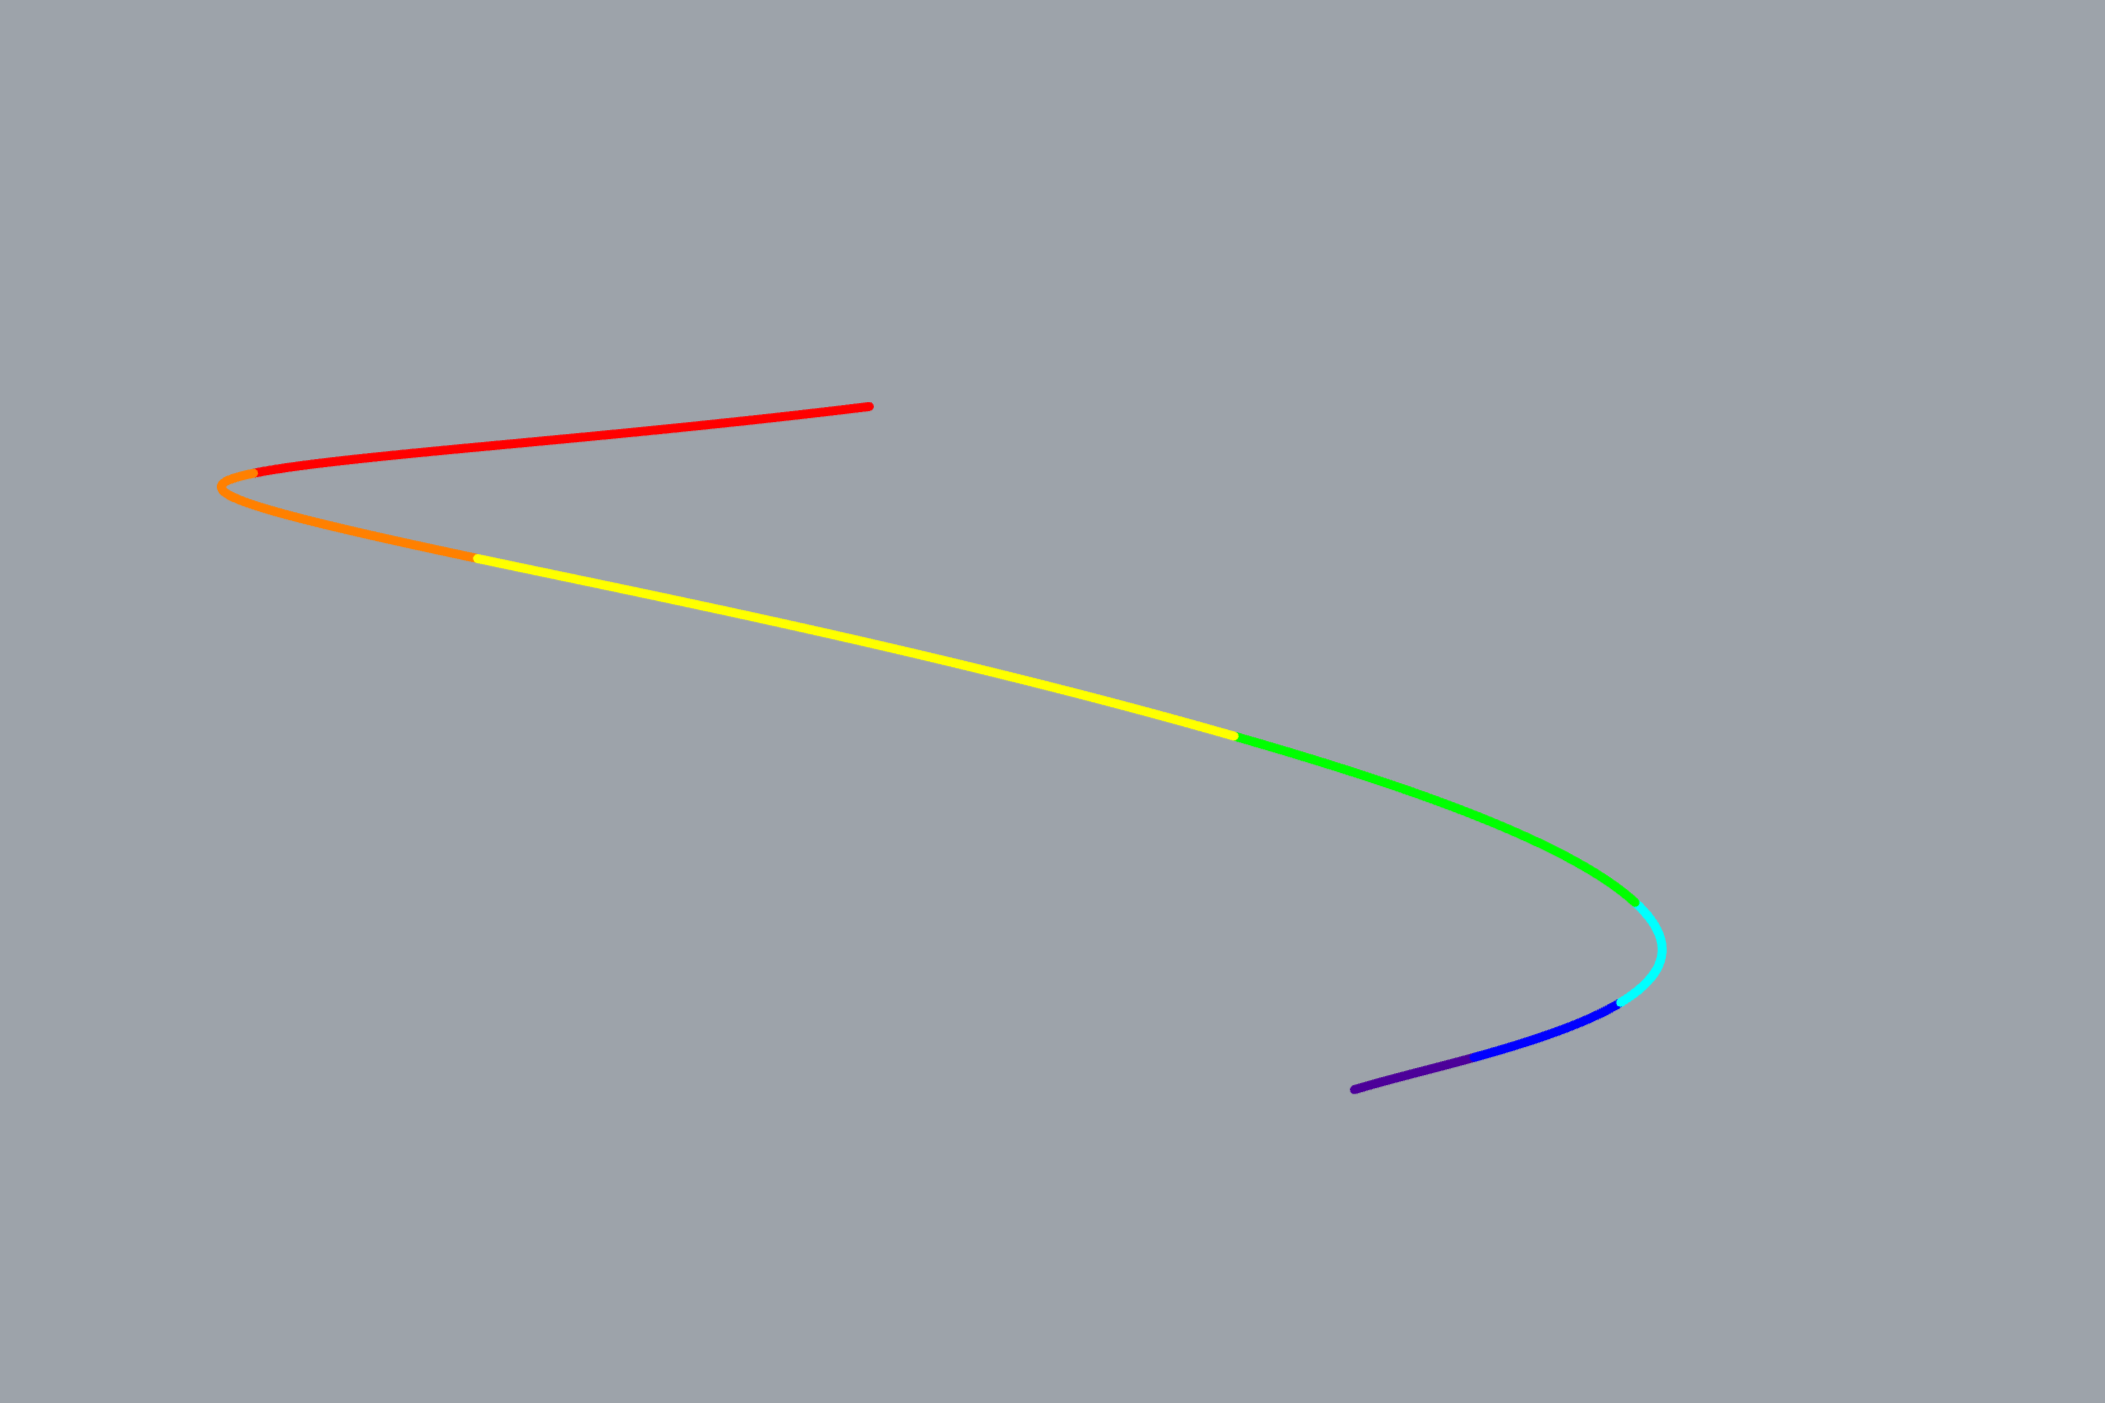
\includegraphics[width=\textwidth]{figures/Seven_Color_Bezier.png}\\
				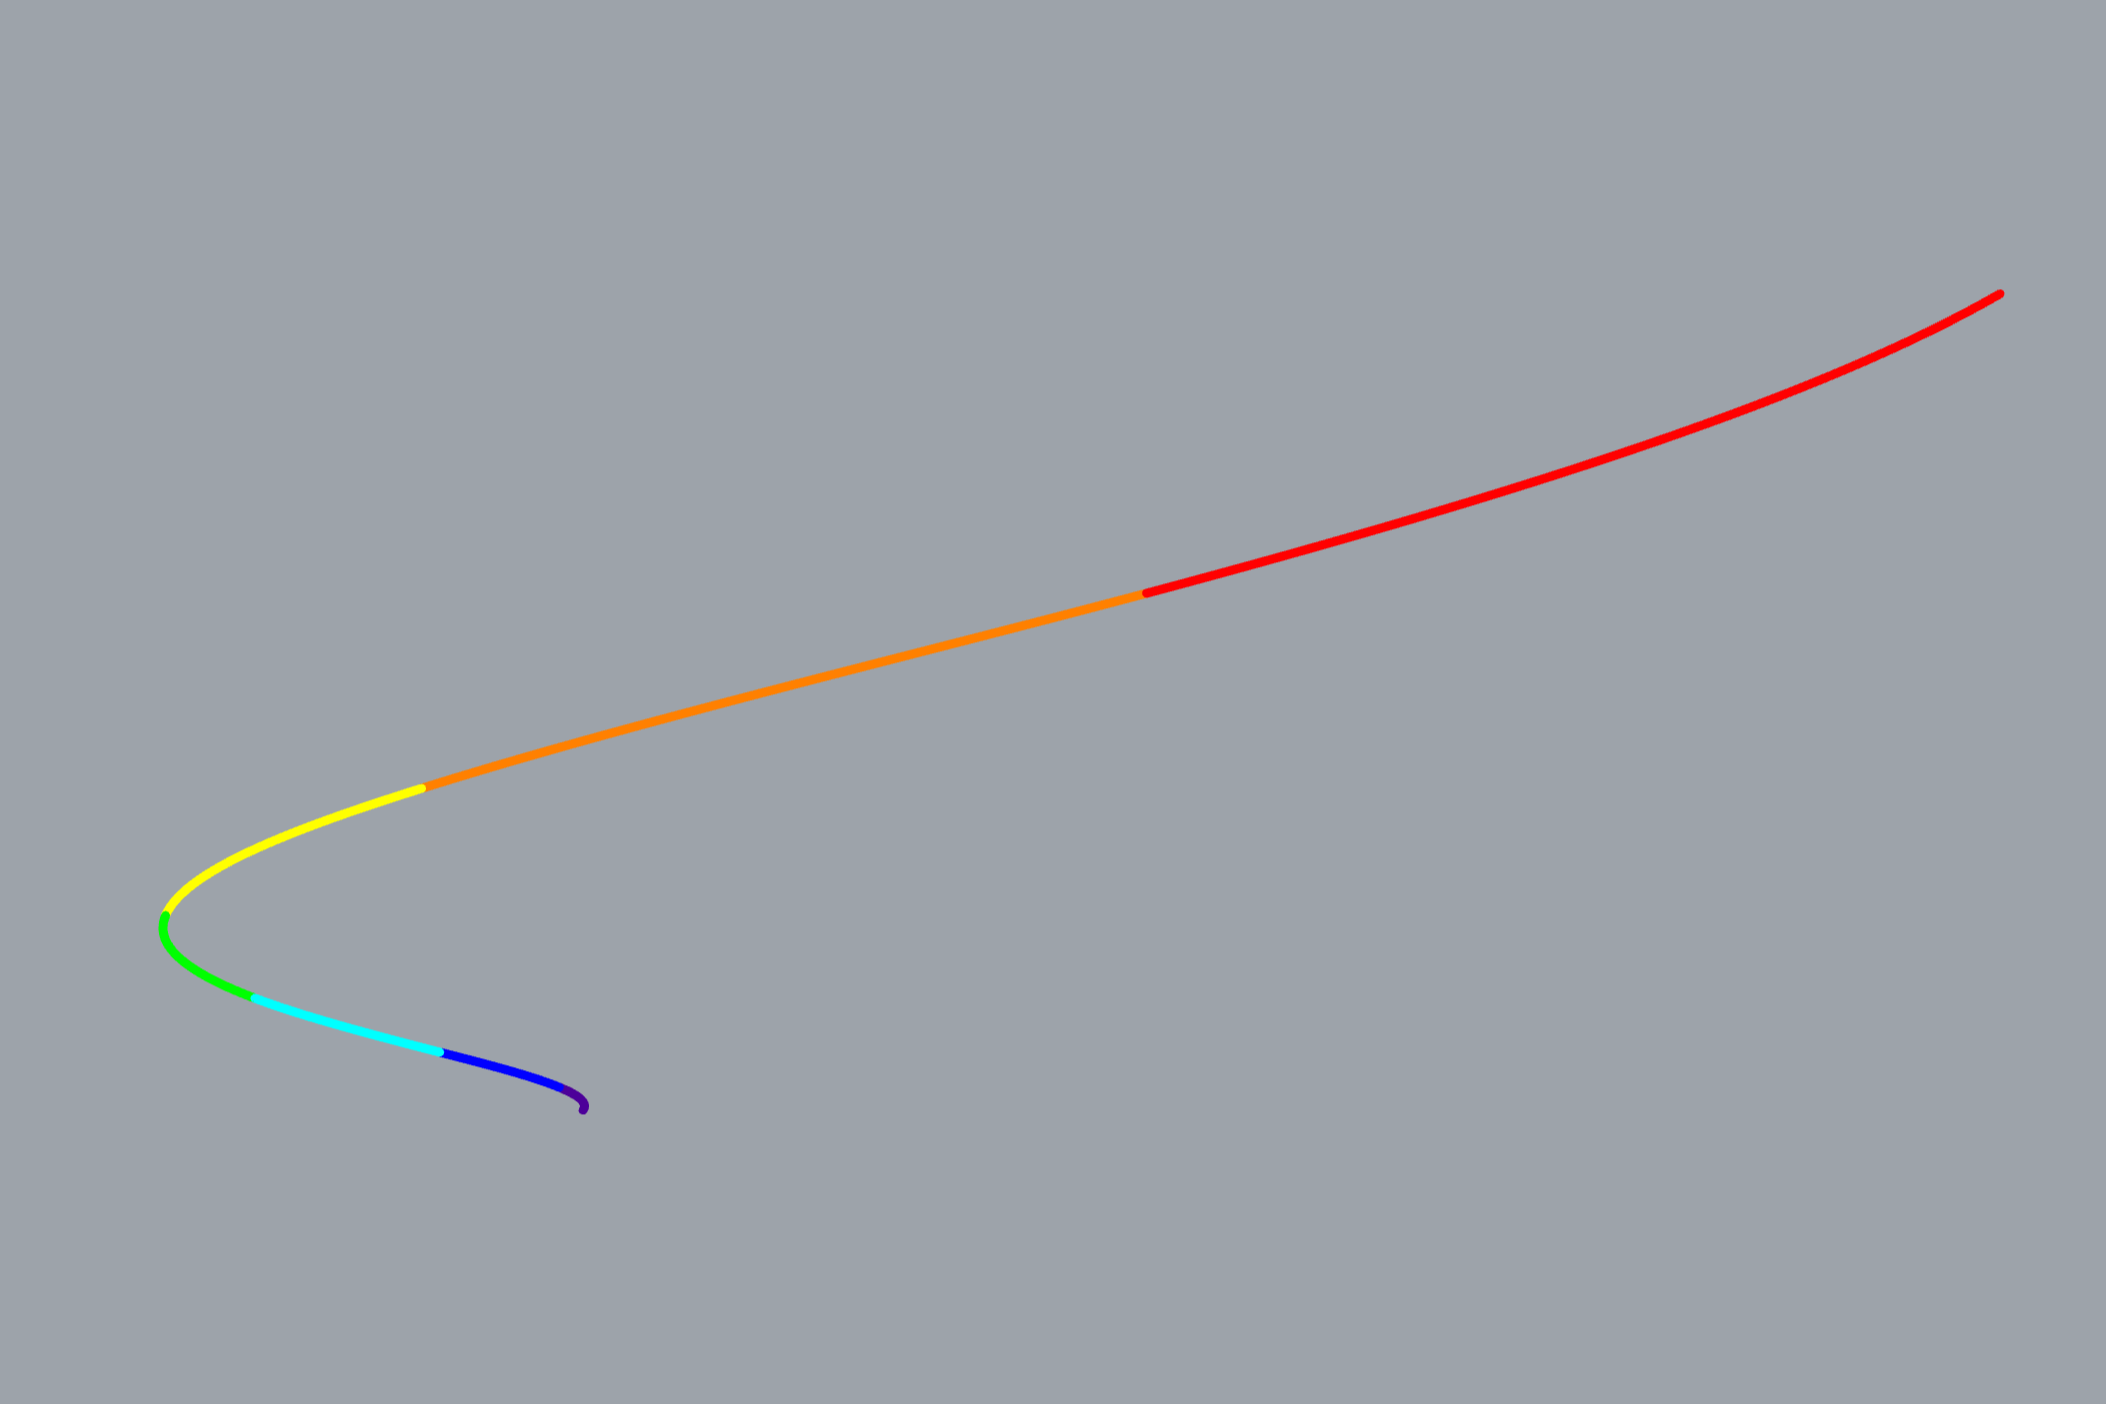
\includegraphics[width=\textwidth]{figures/Seven_Color_Bezier_Front.png}
			\end{minipage}\hfill
			\begin{minipage}[b]{0.45\textwidth} % 右半部分
				\centering
				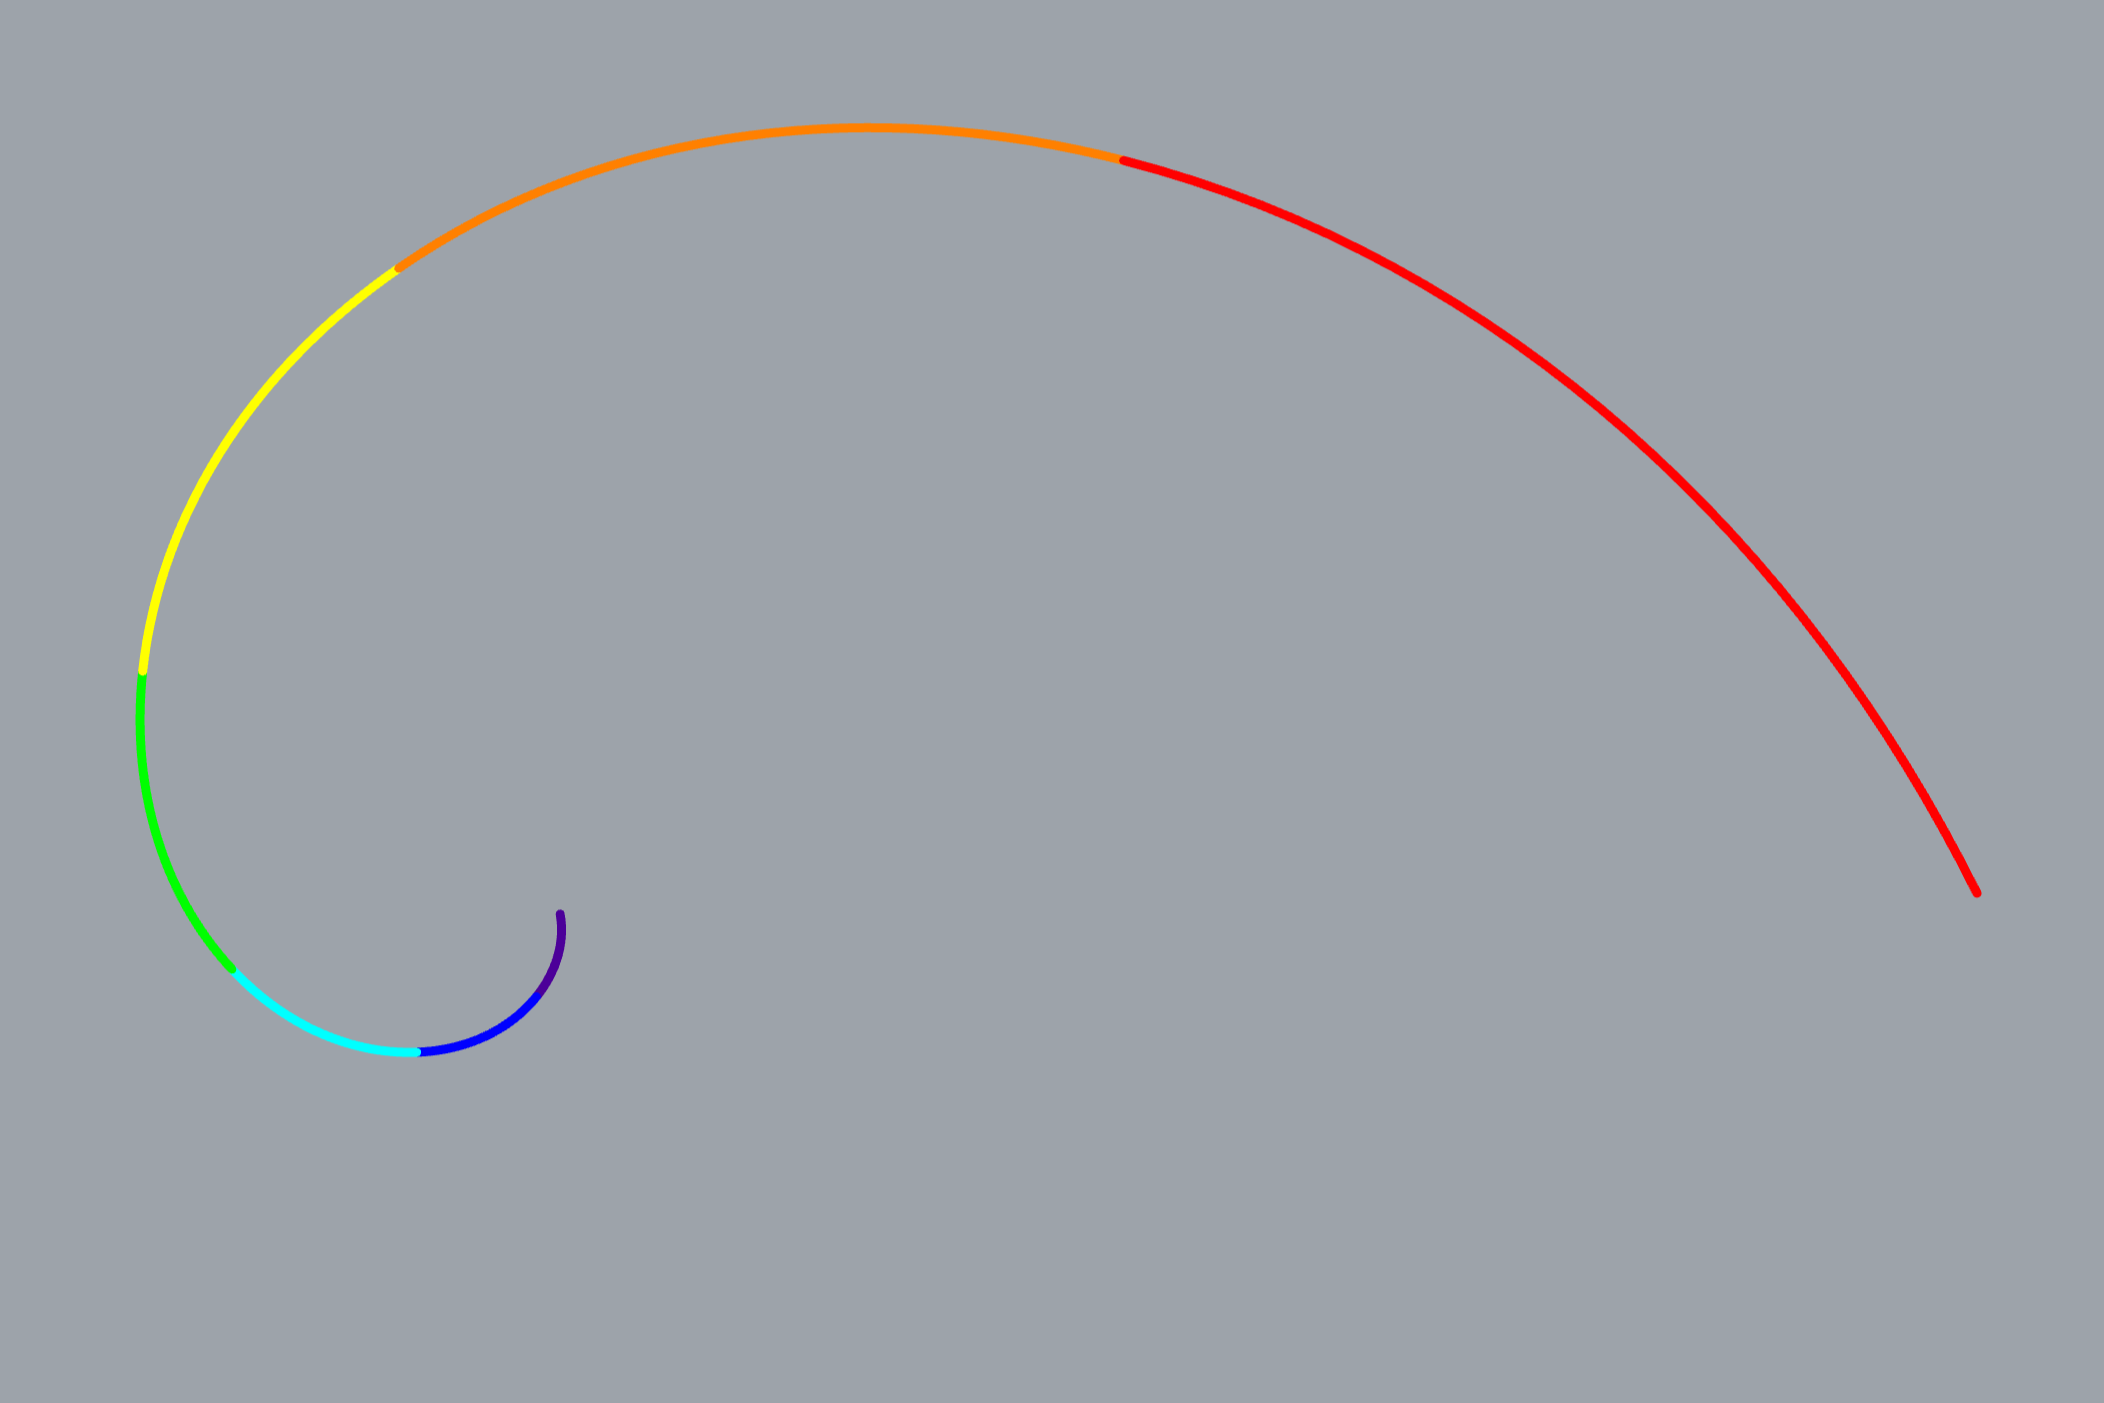
\includegraphics[width=\textwidth]{figures/Seven_Color_Bezier_Top.png}\\
				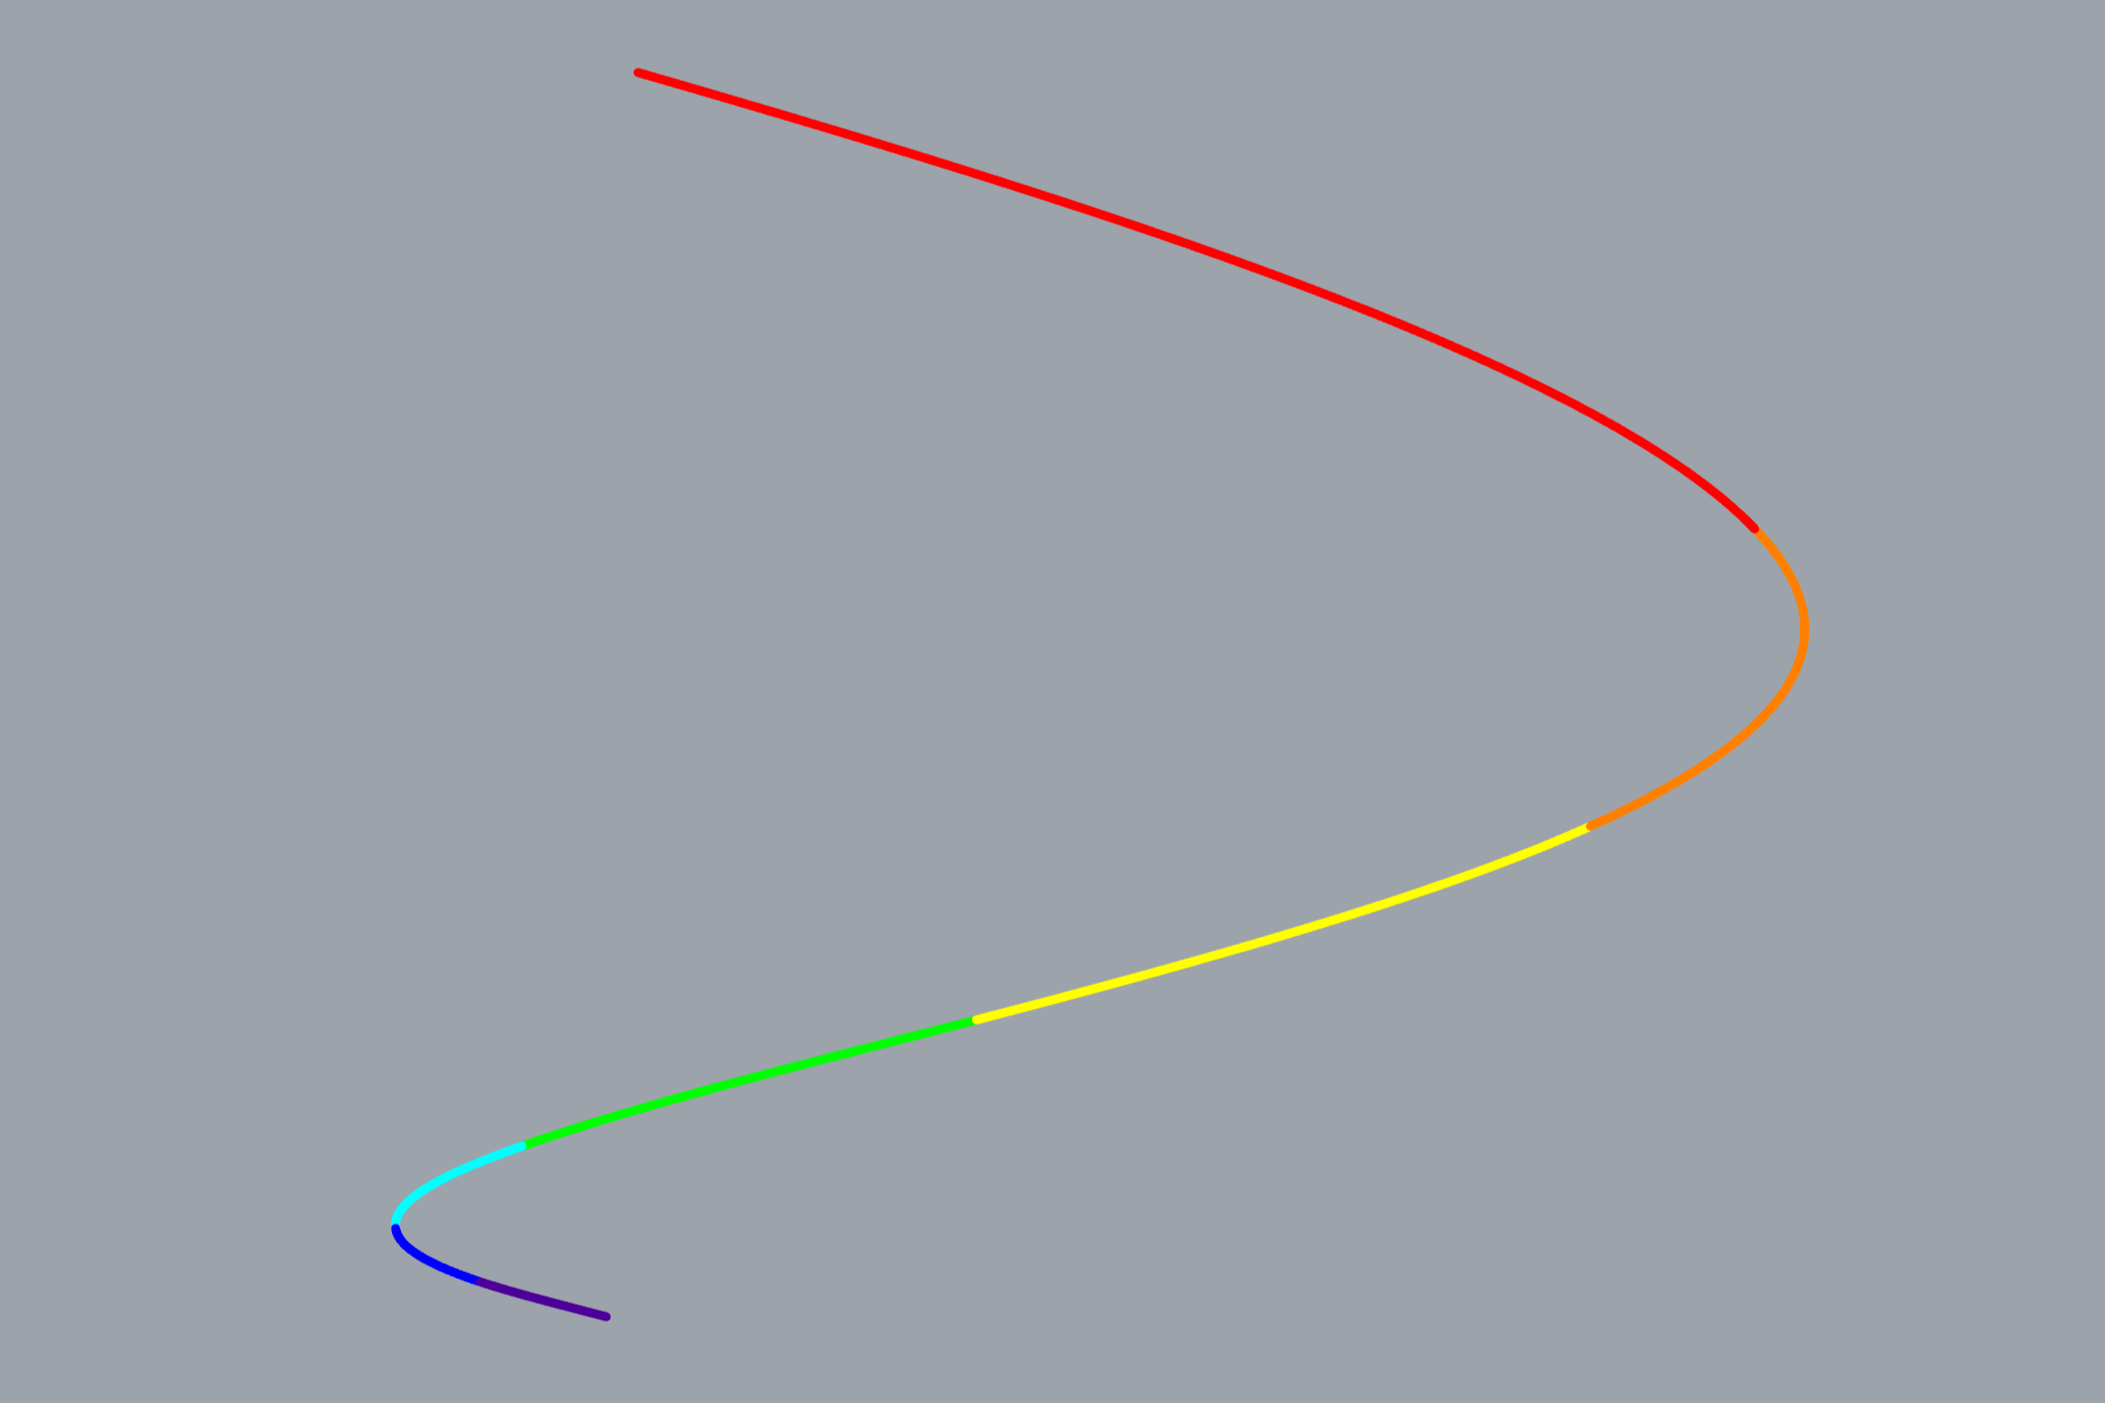
\includegraphics[width=\textwidth]{figures/Seven_Color_Bezier_Right.png}
			\end{minipage}
			\caption{七段Euler B\'ezier曲线$G^1$拼接而成. }
			\label{seven color bezier}
		\end{figure}
		\begin{figure}[ht]
			\centering
			
			\begin{minipage}[b]{0.4\textwidth} % 左半部分
				\centering
				\includesvg[width=\textwidth]{figures/seven_colors_curvature_bezier.svg}
			\end{minipage}\hfill
			\begin{minipage}[b]{0.4\textwidth} % 右半部分
				\centering
				\includesvg[width=\textwidth]{figures/seven_colors_torsion_bezier.svg}
			\end{minipage}
			\caption{左: 图(\ref{seven color bezier})中七段B\'ezier曲线的曲率; 右: 图(\ref{seven color bezier})中七段B\'ezier曲线的挠率. }
			\label{seven color bezier_table}
		\end{figure}
	
	\begin{figure}[h]
		\centering
		\begin{minipage}[b]{0.4\textwidth} % 左半部分
			\centering
			\includesvg[width=\textwidth]{figures/seven_colors_curvature_bspline.svg}
		\end{minipage}\hfill
		\begin{minipage}[b]{0.4\textwidth} % 右半部分
			\centering
			\includesvg[width=\textwidth]{figures/seven_colors_torsion_bspline.svg}
		\end{minipage}
		\caption{左: 图(\ref{seven color bezier})中七段B-spline曲线的曲率; 右: 图(\ref{seven color bezier})中七段B-Spline曲线的挠率. }
		\label{seven color bspline_table}
	\end{figure}
		
		
		\renewcommand\refname{参考文献}
		\addcontentsline{toc}{section}{参考文献}
		\begin{thebibliography}{100}%此处数字为最多可添加的参考文献数量
				\bibitem{article1}第一篇文献.
				\bibitem{article2}第二篇文献.
				\bibitem{article3}第三篇文献.
				\bibitem{article4}第四篇文献.
		\end{thebibliography}  
\end{document}